% !TeX encoding = utf8
% !TeX spellcheck = en_US
% !BIB program = biber
% !TeX program = lualatex


\documentclass[12pt,oneside,letterpaper]{article}

\nonstopmode

% Set a better default text area (note: don't use this and geometry at the same time.)
% \usepackage[DIV=10]{typearea}
\usepackage[margin=1.5in]{geometry}
\usepackage{fontspec}
\defaultfontfeatures{Ligatures=TeX}
\usepackage{amsmath}  % must be loaded before unicode-math
\usepackage{amsthm}
% Libertinus code suggested by https://tex.stackexchange.com/a/364502
\usepackage[
    math-style=ISO,
    bold-style=ISO,
    partial=upright,
    nabla=upright
]{unicode-math}
\setmainfont[Numbers={OldStyle, Proportional}]{Libertinus Serif}
\setsansfont{Libertinus Sans}
\setmathfont{Libertinus Math}
\newfontface\titlefont{Libertinus Serif Display}[Numbers={OldStyle, Proportional}, Fractions=Off,Ligatures=Common]
\newfontface\textfracfont{Libertinus Serif}[Numbers={OldStyle, Proportional}, Fractions=On]
\newfontface\tabularoldstylefont{Libertinus Serif}[Numbers={OldStyle, Monospaced}, Fractions=Off]

\usepackage{csquotes}
\usepackage[final]{microtype}
\frenchspacing{}
\microtypecontext{spacing=french}

% Don't do ligatures in compound words:
\usepackage[english]{selnolig}

\usepackage{ragged2e}  % allow for ragged-right with hyphenation


% Format sections:
% \titleformat{command}[shape]{format}{label}{sep}{before-code}[after-code]
\usepackage[it, small]{titlesec}

% Format itemized lists
\usepackage{enumitem}
\setlist{nolistsep} % more aggressive than noitemsep

% allow page breaks in math equations
\allowdisplaybreaks

\newcounter{axiomcounter}
\newcounter{theoremcounter}
\newcounter{examplecounter}
\newcounter{propositioncounter}
\newcounter{lemmacounter}
\newcounter{corollarycounter}

% Make it easier to change the spacing around these math environments
\newlength{\premathenv}
\setlength{\premathenv}{0.2\baselineskip}
\newlength{\withinmathenv}
\setlength{\withinmathenv}{0\baselineskip}
\newlength{\postmathenv}
\setlength{\postmathenv}{\premathenv} % default to the same, but could change.


\newcommand{\norm}[1]{\left\lVert#1\right\rVert}
\newcommand{\length}[1]{\left\lvert#1\right\rvert}

\theoremstyle{definition}
\newenvironment{theorem}[1]{%
\vspace{\premathenv}%
\refstepcounter{theoremcounter}%
\noindent\textbf{Theorem \thetheoremcounter}
{#1}
\vspace{\withinmathenv}
}{% end of beginning of environment, beginning of end of env
\vspace{\postmathenv}%
}
\newenvironment{proposition}[1]{%
\vspace{\premathenv}%
\refstepcounter{propositioncounter}%
\noindent\textbf{Proposition \thepropositioncounter}
{#1}
\vspace{\withinmathenv}
}{% end of beginning of environment, beginning of end of env
\vspace{\postmathenv}%%
}
\newenvironment{lemma}[1]{%
\vspace{\premathenv}%
\refstepcounter{lemmacounter}%
\noindent\textbf{Lemma \thelemmacounter}
{#1}
\vspace{\withinmathenv}
}{% end of beginning of environment, beginning of end of env
\vspace{\postmathenv}%
}
\newenvironment{corollary}[1]{%
\vspace{\premathenv}%
\refstepcounter{corollarycounter}%
\noindent\textbf{Corollary \thecorollarycounter}
{#1}
\vspace{\withinmathenv}
}{% end of beginning of environment, beginning of end of env
\vspace{\postmathenv}%
}
\newenvironment{axiom}[1]{%
\vspace{\premathenv}%
\refstepcounter{axiomcounter}%
\noindent\textbf{Axiom \theaxiomcounter}
{#1}
\vspace{\withinmathenv}
}{% end of beginning of environment, beginning of end of env
\vspace{\postmathenv}%
}
\newenvironment{example}[1]{%
\vspace{\premathenv}%
\refstepcounter{examplecounter}%
\noindent\textbf{EXAMPLE \theexamplecounter}
{#1}
\vspace{\withinmathenv}
}{% end of beginning of environment, beginning of end of env
\vspace{\postmathenv}%
}

\renewenvironment{proof}{%
\vspace{\premathenv}% previously \vspace{1\baselineskip}
\noindent{\textit{Proof:} }
}{% end of beginning of environment, beginning of end of env
\qed
\vspace{\postmathenv}% previously \vspace{1\baselineskip}
}
\newtheorem{case}{Case}
\renewcommand*{\thecase}{\Alph{case}}
\newtheorem{assumption}{Assumption}
\renewcommand*{\theassumption}{\Alph{assumption}}

\def\equationautorefname~#1\null{(#1)\null}

\newcounter{auditpolicy}
\setcounter{auditpolicy}{-1}
\newenvironment{auditpolicy}[1]{%
\refstepcounter{auditpolicy}%
{\tabularoldstylefont(\theauditpolicy)}~#1%
}


\usepackage{fancyhdr}
\pagestyle{fancy}
\lhead{}
\chead{}
\rhead{}
\lfoot{}
\cfoot{}
\rfoot{\thepage}
\renewcommand{\headrulewidth}{0pt}
\usepackage{xcolor}

% Redefine \left and \right with better spacing
\usepackage{mleftright}
\mleftright{}

% Define \expected and \indicator commands
\DeclareMathOperator{\blackboardE}{\mathbb{E}}
\newcommand{\expected}[1]{\blackboardE\left[#1\right]}
\newcommand{\indicator}[1]{\symbf{1}\left[#1\right]}



\usepackage{rotating} % provide the sidewaysfigure environment

% Set up tables
\usepackage[online,flushleft]{threeparttable}
\usepackage{dcolumn}
\newcolumntype{d}{D{@}{\hspace{0pt}}{4}}
\newcommand{\textcol}[1]{\multicolumn{1}{c}{#1}}

\usepackage{sparklines}
\usepackage{tabularx}
\usepackage{booktabs}

% Bibliograph
\usepackage[
  authordate,
  isbn=false,
  backend=biber,
  autopunct=true,
  backref=true
]{biblatex-chicago}
\renewcommand*{\bibfont}{\small}
\addbibresource{refs.bib}
\addbibresource{data_cites.bib}
\addbibresource{methane_measurement_refs.bib}

% use the \ce{} command for chemistry expressions like \ce{CO2}
\usepackage[version=4]{mhchem}

\usepackage{nameref}

% Set up a boolean so we can easily turn endfloat on and off.
% To turn on, change to \setboolean{endfloat}{true}
\usepackage{ifthen}

\newboolean{endfloat}
\setboolean{endfloat}{false}
\ifthenelse{\boolean{endfloat}}{
  \usepackage{endfloat}
  % stopendfloat from putting everything on separate pages
  \renewcommand{\efloatseparator}{\mbox{}}
}{ % else :
  \usepackage{placeins} % provide \FloatBarrier command
}

\usepackage{graphicx}
\graphicspath{{../graphics/}}
\usepackage{import} % better relative import paths
\usepackage{tikz}
\usetikzlibrary{calc}
%\usepackage{gitinfo2}  % requires git hooks!  See the code/git_hooks folder in this repo.
\usepackage{wrapfig} % provides wrapfigure and wraptable environments


% Define a command \blfootnote (blind foodnote or blank footnote)
% Redefine \thefootnote to remove the symbol
% Redefine \@makefntext to try to mimic the biblatex-chicago option footmarkoff, but only for the scope of this command.
% Then reset the counter.
\makeatletter
\newcommand{\blfootnote}[1]{%
  \begingroup
  \renewcommand{\thefootnote}{}%
  \renewcommand{\@makefntext}{}%
  \footnote{#1}%
  \addtocounter{footnote}{-1}%
  \endgroup
}
\makeatother


% Add an orcid logo:
% Borrowed partly from https://tex.stackexchange.com/a/445583
% And downloaded graphic from
% https://figshare.com/articles/ORCID_iD_icon_graphics/5008697
\usepackage{scalerel}
\newcommand\orcidicon[1]{\href{https://orcid.org/#1}{\mbox{\scalerel*{

\includegraphics{ORCIDiD_iconvector.pdf}
}{|}}}}


% Run texcount shell command and input result. Requires shell escape (or restricted shell escape) and associated security warnings
% The -merge option includes counts for any \input{}-ed files.
\usepackage{shellesc}
\newcommand{\wordcount}[1]{%
\input|"texcount -1 -sum -merge -q #1.tex"%
}

\newcommand{\thoughtbreak}{%
\begin{center}
\rule{5em}{1pt}
\end{center}
}

% \usepackage[modulo]{lineno}
% \linenumbers
% \usepackage[onehalfspacing]{setspace}
\usepackage{setspace}
\onehalfspacing

% Ensure more achievable output (font embedding etc.) but see the docs about
% what it takes to be PDF/A-3b compliant.
% \usepackage[a-3b]{pdfx}
\usepackage{hyperref}

% Write out acronyms in small caps that can be copy-pasted as full caps.
% It would be nice to have something that depended less on defining each acronym, or less on the c2sc OpenType font feature
% Usage: \makeacronym{NASA}
\usepackage{accsupp}
\usepackage{glossaries}
\glsdisablehyper{} % disable hyperlinks


% Create acronyms in a way that works nicely with smallcaps.
% (eg \setacronymstyle{long-sc-short})
% This code makes the acronym lowercase so small caps can be applied,
% but adds an accessibility layer so it copies-pastes in upper case.
\newcommand{\makeacronym}[2]{%
\newacronym{#1}{%
\protect\BeginAccSupp{method=plain,ActualText=#1}%
\MakeLowercase{#1}%
\protect\EndAccSupp{}%
}{#2}%
}
\makeacronym{ARE}{Agricultural and Resource Economics}
\makeacronym{AVIRIS-NG}{``next generation airborne visible/infrared imaging spectrometer''}
\makeacronym{BAU}{business as usual}
\makeacronym{BLS}{Bureau of Labor Statistics}
\makeacronym{CDD}{cooling degree days}
\makeacronym{CDF}{cumulative distribution function}
\makeacronym{CEMS}{continuous emissions monitoring}
\makeacronym{CI}{confidence interval}
\makeacronym{DBSCAN}{density-based spatial clustering of applications with noise}
\makeacronym{DWL}{deadweight loss}
\makeacronym{EPA}{Environmental Protection Agency}
\makeacronym{EU ETS}{European Union Emission Trading Scheme}
\makeacronym{FOC}{first-order condition}
\makeacronym{GDP}{gross domestic product}
% \makeacronym{FEAST}{}
% Could make GHG have a proper plural: https://tex.stackexchange.com/a/128419
\newacronym[longplural={greenhouse gases}, shortplural={ghg}]{GHG}{%
\protect\BeginAccSupp{method=plain,ActualText=GHG}%
ghg%
\protect\EndAccSupp{}
}{greenhouse gas}
\makeacronym{GHGI}{greenhouse gas inventory}
\makeacronym{GHGRP}{greenhouse gas reporting program}
\makeacronym{GOSAT}{Greenhouse Gases Observing Satellite}
\makeacronym{GWP}{global warming potential}
\makeacronym{HDD}{heating degree days}
\makeacronym{i.i.d.}{independent and identically distributed}
\makeacronym{IHS}{inverse hyperbolic sine}
\makeacronym{IPCC}{Intergovernmental Panel on Climate Change}
\makeacronym{KKT}{Karush–Kuhn–Tucker}
\makeacronym{LDAR}{leak detection and repair}
\makeacronym{MCMC}{Markov chain Monte Carlo}
\makeacronym{MLE}{maximum likelihood estimation}
\makeacronym{MSE}{mean squared error}
\makeacronym{OSHA}{Occupational Safety and Health Administration}
\makeacronym{PDF}{probability density function}
\makeacronym{SCC}{social cost of carbon}
\makeacronym{SDID}{synthetic difference in differences}
\makeacronym{SNL}{SNL Financial}
\makeacronym{WAIC}{widely applicable information criterion}
 % loads glossaries package, and should be loaded after hyperref
\setacronymstyle{long-sc-short}

\hypersetup{colorlinks,
  linkcolor=blue!40!black,
  filecolor=black,
  urlcolor=blue!40!black,  % 40% blue, 60% black
  citecolor=black,
  pdfpagemode=UseNone,
  pdftoolbar=false,
  pdftitle={},
  pdfauthor={},
  pdfsubject={},
  pdfcreator={},
  pdfproducer={},
  pdflang=en,
  unicode=true
}
\widowpenalty 9999

\begin{document}
\begin{refsection}
\begin{center}

\
{\LARGE\titlefont
Hard to Measure Well:
\vspace{6pt}

Can Feasible Policies Reduce Methane Emissions?
}
\vspace{1.5\baselineskip}


{\Large\titlefont
Karl Dunkle Werner%
\textsuperscript{ \orcidicon{0000-0003-0523-7309}}
and Wenfeng Qiu%
\blfootnote{%
\noindent Author affiliations:
US Treasury and UC Berkeley Department of Agricultural and Resource Economics.

\noindent
Contact: \href{mailto:karldw@berkeley.edu}{karldw@berkeley.edu} and
\href{mailto:wqiu03@berkeley.edu}{wqiu03@berkeley.edu}.

\noindent
We are deeply grateful for the insightful advice and feedback we've received from
faculty and students in the Energy Institute at Berkeley,
Daniel Cusworth,
Kelsey Foster,
Christian Frankenberg,
Catie Hausman,
Larry Karp,
Ryan Kellogg,
Susan Powell,
Evan Sherwin,
Andrew Thorpe,
Hannah Yung,
and our wonderful PhD cohort.
We also appreciate great research assistance from Shuyi Deng.
All errors are, of course, our own.
Karl is grateful for the generous support of the Alfred P. Sloan Foundation Pre-doctoral Fellowship on Energy Economics, awarded through the NBER.
The views and findings presented this research do not necessarily represent the views of the US Treasury or any other author affiliation.

\noindent
Code for this paper is available: \url{https://github.com/karldw/paper_hard_to_measure_well}.\\
} % end of footnote
}% end of \Large\titlefont

{\large\titlefont
\vspace{1\baselineskip}

\today{}

%(\wordcount{paper} words)\\
}% end of \large\titlefont

\end{center}




\begin{abstract}
\begin{singlespace}
  \noindent
% Long abstract:
% Oil and gas wells emit large quantities of methane, a greenhouse gas 30~times more potent than carbon dioxide.
% Methane emissions are rarely priced and lightly regulated---in part because they are hard to measure---leading to a large climate externality.
% However, measurement technology is improving, with remote sensing and other techniques opening the door for policy innovation.
% We present a theoretical model of emissions abatement at the well level and a range of feasible policy options, then use data constructed from cross-sectional scientific studies to estimate abatement costs.
% We simulate audit policies under realistic constraints, varying the information the regulator uses in choosing wells to audit.
% These policies become more effective when they can target on well covariates, detect leaks remotely, and charge higher fees for leaks.
% % Goal here: make clear that the policy specifics matter, and the lessons here are important for methane and other policy.
% We estimate that a policy that audits 1\% of wells with uniform probability achieves less than 1\% of the gains of the infeasible first best.
% Using the same number of audits targeted on remotely sensed emissions data achieves gains of 30--60\% of the first best.
% These results demonstrate that, because leaks are rare events, targeting is essential for achieving welfare gains and emissions reductions.
% Auditing a small fraction of wells can have a large impact when properly targeted.

% 100-word abstract:
\noindent
Oil and gas wells emit methane, a potent greenhouse gas.
Emissions are minimally regulated, leading to a large climate externality.
We present a theoretical model of emissions abatement and feasible policy options, estimate abatement costs using cross-sectional data from scientific studies, then simulate policies under realistic constraints.
Because large leaks are rare, targeting is essential for achieving policy goals.
A policy that audits 1\% of wells with uniform probability achieves less than 1\% of the gains of the infeasible first best, while targeting audits using remotely sensed emissions can achieve 30--60\% of the first best.

\noindent \textsc{jel: c54, h23, k32, q55, q58}
\end{singlespace}
\end{abstract}

% Longer list of relevant JEL codes.
% C31 Multiple Variables : Cross-Sectional Models, Spatial Models, Treatment Effect Models, Quantile Regressions, Social Interaction Models
% C54: Quantitative Policy Modeling
% H23  Taxation, Subsidies, and Revenue: Externalities, Redistributive Effects, Environmental Taxes and Subsidies
% K32  Other Substantive Areas of Law: Energy, Environmental, Health, and Safety Law
% L51  Economics of Regulation
% L71  Industry Studies: Mining, Extraction, and Refining: Hydrocarbon Fuels
% Q48  Energy: Government Policy
% Q52  Environmental Economics: Pollution Control Adoption and Costs, Distributional Effects, Employment Effects
% Q55  Environmental Economics: Technological Innovation
% Q58  Environmental Economics: Government Policy

\newpage


\newpage

\section{Introduction}
\label{sec:introduction}


Oil and gas wells emit large quantities of methane, a powerful greenhouse gas with the second largest impact after carbon dioxide.
Methane accounts for roughly one-tenth of total \gls{GHG} emissions, though its contribution is measured much less precisely than carbon dioxide's.
Fossil fuels, particularly oil and natural gas, are the largest human-driven sources of methane \parencite{epa-ghgi:2020, Alvarez/etal:2018}.
As fracking has dramatically increased US oil and natural gas production, methane emissions have followed, and these emissions are now roughly the same magnitude as the emissions from all fuel used in the western US electricity grid \parencite{epa-egrid-2018}.
Natural gas has been heralded as a cleaner substitute for coal and a bridge fuel in the transition to a low carbon economy.
However, if these methane emissions are large enough, natural gas may emit more \gls{GHG} than coal.%
\footnote{%
The lifecycle \gls{GHG} emissions of natural gas may be lower than coal as long as the total leakage rate is below 5--10\% \parencite{Hausfather:2015}.
We focus on upstream leakage from wells, where 1--4\% of gas leaks out.
Emissions from pipelines and end users also contribute significantly, and further quantifying all of these remains an active field of research.
}
Beyond debates over coal and natural gas, these leaks increase both the lifecycle \gls{GHG} emissions of gasoline and the relative value of renewable energy.


Measuring methane is costly---it's infeasible to put a continuous emissions monitor on every well---so pricing emissions is challenging.
The standard economic prescription in this case would be to audit infrequently and charge a high fine, so that the expected penalty is equal to the social cost (plus enforcement costs).
This approach has theoretical appeal, but is infeasible because of legal and logistical constraints.
The constraints on fees range from the backstop of bankruptcy, to legal doctrine limiting punitive damages, to political pushback \parencite{Boomhower:2019, exxon_v_baker:2008}.
Currently, no US jurisdiction charges a price for methane emissions
\parencite{Rabe/Kaliban/Englehart:2020}.

This paper combines an economic model with empirical estimates in order to quantify the potential gains from \emph{feasible} audit policies and to demonstrate the value of remotely sensed data that could improve audit targeting.
We account for real-world constraints on policies that can be enacted and the information available to the regulator.
These constraints take the form of limits on the fees that can be charged, the regulator's capacity to conduct audits, and the fidelity and detection threshold of the remotely sensed measurements.
Policies under these constraints offer some improvement over the benchmark of no policy,
but the gains vary dramatically, depending on the fee the regulator can charge and the remote sensing information available.


We note that imperfect measurement is not isolated to methane, or even environmental economics.
Enforcing any policy requires measurement.
The quality and cost of these measurements determine which policies are feasible.
In recent decades, remote sensing, administrative data, and other indirect information have improved dramatically, raising the possibility that policy can be based on or informed by these measures.
At the same time, and despite a great deal of excitement about remote sensing, policies that make direct use of these tools are rare.
Our work highlights a promising case where they could be applied, while acknowledging the measurements' limits for enforcing policy.
We integrate a theoretical model, tailored to our data setting, with a newly constructed dataset and Bayesian structural estimation to evaluate the gains a constrained regulator could achieve with additional information.

To start our analysis, we develop a theoretical model of abatement and welfare.
Using the model, we consider how well operators would change their behavior in response to a feasible but imperfect audit policy---one where the expected fee for emitting differs from the social cost,
and may be zero for some wells because of measurement or auditing limitations.

In our model, and consistent with the scientific literature, large leaks are the result of stochastic process failures
\parencite{Lyon/Alvarez/Zavala-Araiza/Brandt/Jackson/Hamburg:2016, ZavalaAraiza/etal:2017}.
These leaks are rare and hard to predict, but large sources of \gls{GHG}.
Well operators can reduce the duration of leaks by checking wells more frequently and the occurrence of new leaks by investing in routine maintenance and better equipment.
We assume well operators abate expected emissions by reducing the \emph{probability} a well is leaking at any given moment, rather than reducing the size of leaks.
Our stylized model yields closed-form solutions for welfare and abatement as functions of the leak size distribution and the well operators' cost parameters.
We parameterize the model flexibly, using data on leaks at the well pad level.\footnote{%
A well pad is a group of one or more closely spaced wells, typically within a few yards of one another.
}
To construct the distribution of emissions, we combine several datasets from different scientific teams.
We match these leakage measures to specific well pads, and we estimate the fraction that have detectable emissions.
Our main dataset uses emissions estimates collected by airplanes flying over approximately 15,000 well pads in California, New Mexico, and Colorado.
We use the variation in leak size and presence to infer the distribution of sizes when leaks occur, as well as the well operator' costs of preventing those leaks.


In addition to being a greenhouse gas, methane is also the primary component of natural gas.
To leak methane into the atmosphere is to lose the commodity value of the gas,
which provides a private incentive to abate.
However, because the commodity price is less than one-tenth the value of social damages from leaking, well operators don't face a strong enough incentive to abate to the socially optimal level.
We use this private incentive to learn as much as possible in the absence of policy.
We build our model assuming well operators are avoiding leaks optimally, given this weak private incentive, then consider how behavior would change if the well operator faced some expected fee for emissions.

When we discuss audits, we consider on-the-ground measurements.
When a well is audited, we assume the regulator has to drive to the well and take downwind measurements of the well's emissions using standard methods approved by the \gls{EPA}.
These on-the-ground measurements may be necessary, even when leaks can be measured remotely, because of noise in the remote sensing or regulatory constraints.


To think about a range of audit policies, we compare five cases:

\begin{auditpolicy}
\label{policy-bau}
no audits, the status quo,
\end{auditpolicy}
\begin{auditpolicy}
\label{policy-uniform}
audit every well with equal probability,
\end{auditpolicy}
\begin{auditpolicy}
\label{policy-target-x}
target audits based on well covariates,
\end{auditpolicy}
\begin{auditpolicy}
\label{policy-target-e}
measure leaks remotely, using that information to target audits, and
\end{auditpolicy}
\begin{auditpolicy}
\label{policy-remote}
measure leaks remotely and, without auditing, assess fines based on measurements.
\end{auditpolicy}
\noindent Assessing fines on the basis of remote measurements (policy~\ref{policy-remote}) is infeasible in current legal structures, but provides an interesting point of comparison.

Comparing each of the audit policies (\ref{policy-uniform}--\ref{policy-target-e})
with the status quo (policy~\ref{policy-bau}) allows us to think about the gains available from an audit-type policy.
Comparing policy~\ref{policy-target-e}, which uses remote sensing, with policies \ref{policy-uniform} and \ref{policy-target-x}, which don't, provides information about the scope for policy innovation with these new tools.
Charging fees based on remote sensing alone (policy~\ref{policy-remote}) provides an infeasible benchmark, and could achieve the first-best under additional assumptions.
Each of these policies implies some expected value of the fee a well operator would pay.
In our model, we will consider the deadweight loss that arises from the regulator not being able to set the expected fee to the social cost of emissions.

In the policies that use remotely sensed data, and in any policy that depends on measurement, the effectiveness of the policy depends on the quality of the measurement.
For our context, the detection threshold is an important concern---with a high threshold, only the largest leaks will be detected remotely.
In our analysis, we assume these measurements are available from methane-observing satellites, using realistic values of their detection capacity
\parencite{Cusworth/Jacob/Varon/Miller/Liu/Chance/Thorpe/Duren/Miller/Thompson/Frankenberg/Guanter/Randles:2019}.


These are relatively simple policies.
Although they do not offer the theoretical gains of dynamic enforcement or sophisticated mechanism design, they do allow us to focus on the gains that are possible under
feasible policies, and how outcomes change as technological innovation makes more information available
(cf.
\cite{Blundell/Gowrisankaran/Langer:2020, Cicala/Hemous/Olsen:2019, Oestreich:2017}).
We use these policies as tools to think about the space of potential pricing options, and how that space is changed with the availability of remotely sensed measurements.


We estimate that audit policies yield gains over the status quo of no fees.
These gains vary dramatically with the fee amount and the specifics of the policy.
The different policies we consider translate into different expected fees for emitting.
For instance, the uniform audit policy has the same expected fee for every well, and that fee increases as the audit probability or allowed penalty increases.
For a mid-level penalty and 1\% audit budget, the average of the expected fee for emitting is
\$\import{tex_fragments/}{OUTCOME=fee_mean_RULE=uniform_FRAC=1pct_tauT=med-3month.tex} per ton of carbon dioxide equivalent (\ce{CO2e}),
which leads to improving \gls{DWL} by
\import{tex_fragments/}{OUTCOME=welfare_gain_pct_RULE=uniform_FRAC=1pct_tauT=med-3month.tex}
of the difference between the no-fee outcome and the Pigouvian first best.%
\footnote{
Throughout this paper, we use a \ce{CO2e} conversion factor of 29.8, the standard 100-year \gls{GWP} from the \gls{IPCC} \parencite{ipcc_ar6_methane_gwp}.
There is a lively debate, e.g. \textcite{Allen/Shine/Fuglestvedt/Millar/Cain/Frame/Macey:2018}, about the correct way of comparing emissions of different greenhouse gases.
The most internally consistent approach would be to use a \gls{SCC} and social cost of methane.
Using the existing \gls{SCC} estimates, the implied conversion between one ton of \ce{CH4} and one ton of \ce{CO2} ranges from 25.8 to 45.
Alternatively, 100-year \gls{GWP} is approximately consistent with a 3\% discount rate on climate damages
\parencite{Sarofim/Giordano:2018, Mallapragada/Mignone:2019}.
All of these estimates come with uncertainty -- the most recent GWP estimate is 29.8 $\pm$ 11 -- but in our calculations, we assume they're exact.
}
In this scenario, average emissions would fall by
\import{tex_fragments/}{OUTCOME=emission_reduce_tonCO2e_RULE=uniform_FRAC=1pct_tauT=med-3month.tex}
\ce{CO2e} per well per year.
With the same audit budget and penalty, we can also consider a policy that targets on well covariates, rather than auditing with uniform probability.
In this case, the average fee is
\$\import{tex_fragments/}{OUTCOME=fee_mean_RULE=target_x_FRAC=1pct_tauT=med-3month.tex} (mechanically the same as the uniform policy), but is now heterogeneous across wells, with an interdecile range of
\$\import{tex_fragments/}{OUTCOME=fee_p10_RULE=target_x_FRAC=1pct_tauT=med-3month.tex}--%
\import{tex_fragments/}{OUTCOME=fee_p90_RULE=target_x_FRAC=1pct_tauT=med-3month.tex}.
Now the improvement in \gls{DWL} is
\import{tex_fragments/}{OUTCOME=welfare_gain_pct_RULE=target_x_FRAC=1pct_tauT=med-3month.tex},
and the average fall in emissions is
\import{tex_fragments/}{OUTCOME=emission_reduce_tonCO2e_RULE=target_x_FRAC=1pct_tauT=med-3month.tex}.

We can also consider targeting on observed leaks.
We focus on the realistic case where the remote measurement has a high detection threshold, so only the largest leaks are detected.
As we mentioned, in this case the regulator can prioritize wells that were observed leaking, saving some audit effort of auditing wells when they're not leaking.
For the same audit budget and allowed penalty, there's a much higher expected fee:
\$\import{tex_fragments/}{OUTCOME=fee_mean_RULE=target_e_high_FRAC=1pct_tauT=med-3month.tex} per ton \ce{CO2e},
with an interdecile range of
\$\import{tex_fragments/}{OUTCOME=fee_p10_RULE=target_e_high_FRAC=1pct_tauT=med-3month.tex}--%
\import{tex_fragments/}{OUTCOME=fee_p90_RULE=target_e_high_FRAC=1pct_tauT=med-3month.tex}
across wells.

This stronger incentive leads the well operators to abate more, leading to
a \gls{DWL} improvement of
\import{tex_fragments/}{OUTCOME=welfare_gain_pct_RULE=target_e_high_FRAC=1pct_tauT=med-3month.tex},
and average emissions declines of
\import{tex_fragments/}{OUTCOME=emission_reduce_tonCO2e_RULE=target_e_high_FRAC=1pct_tauT=med-3month.tex}.
We also consider other policy options, including different penalties, different fixed audit probabilities, audit probabilities that depend on the cost of auditing, and other policy benchmarks.

These results highlight the importance of both measurement and regulatory constraints.
If there were no limits on the size of fees for leaks, a sufficiently high fine could be employed to induce efficient abatement without targeted audits.
Given realistic constraints on fee amounts and the rarity of leaks, untargeted audits produce very small welfare gains compared to audits that are targeted based on remotely sensed information.
If the allowed fees are severely constrained, even targeted audits yield small gains.

Though the estimates in our paper focus on methane emissions, we view our results as a contribution to several broader literatures.
First, and most directly, we contribute to the discussion of designing and evaluating policy with imperfect measurement.
Second, we contribute to the innovation literature, considering how technological progress in measurement allows for policy innovation.
Third, we compare our results with the small literature on methane abatement.


The challenges of imperfect measurement and imperfect targeting arise in many environmental questions, such as regulating non-point pollution, as well as other economic topics such as tax evasion, teacher value-added and principal--agent problems
\parencite{
Segerson:1988,
Allingham/Sandmo:1972,
Chetty/Friedman/Rockoff:2014,
}.
In all of these areas, if regulators could accurately observe individual actions, they would be able to achieve their goals much more directly.
However, lack of accurate, individual measurement leads to more complicated policies that draw inferences from indirect evidence.
Our research highlights the value of one type of indirect measurement: remote sensing measures that guide on-the-ground audits.\footnote{%
\textcite{AlixGarcia/Millimet:2020} provides a relevant guide to real-world challenges of satellite data, particularly for measuring binary outcomes.
}
We compare the policies that are achievable with and without these additional data.
These additional measurements are a form of innovation, enabling policies that were not previously feasible.
Thus, we contribute to a line of innovation literature that includes \textcite{Nagaraj:2020}, which considers a private-sector case where satellite imagery enabled entry by small firms and changed the structure of the market.

Finally, we're contributing to a relatively small literature on policies to address methane emissions.
\textcite{Ravikumar/etal:2020} is the only study we're aware of that estimates the observed change in methane emissions from a change in policy.
The authors performed repeated surveys of a small number of facilities before and after a \gls{LDAR} program began, and estimate a 44\% reduction in emissions.

Two recent working papers by Levi Marks provide a point of comparison for pricing methane emissions.
\textcite{Marks:2021} estimates the elasticity of methane emissions%
---reported in the \gls{EPA}'s \gls{GHGRP}---%
with respect to  the commodity price of natural gas of methane emissions.
That paper, like ours, estimates abatement costs in the absence of any direct price on emitting methane.
To get around the lack of existing policy, that paper notes that the private incentive to sell natural gas into the commodity market can proxy for a fee on methane emissions.
We rely on the same argument.
Because natural gas prices move in a limited range and are always much lower than the social cost of methane emissions, \textcite{Marks:2021} considers a \$5~per ton \ce{CO2e} tax on emissions to avoid extrapolating too far from the data.
The paper estimates that this tax would result in an emissions reduction of 56\%.
To estimate a comparable policy, we will consider \$5~per ton \ce{CO2e} as the low-end fee a regulator might charge.
We find sharply different results for our \$5 fee, largely because low audit probabilities lead to an expected fee much lower than \$5.
When we consider \emph{expected} fees of approximately \$5, we find results in a similar range, as long as the regulator is able to detect leaks remotely.
For instance, an average fee of
\$\import{tex_fragments/}{OUTCOME=fee_mean_RULE=target_e_high_FRAC=1pct_tauT=med-3month.tex}
per ton of \ce{CO2e}
leads to emissions reductions of
\import{tex_fragments/}{OUTCOME=emission_reduce_tonCO2e_RULE=target_e_high_FRAC=1pct_tauT=med-3month.tex}
\ce{CO2e} per well per year, from a baseline of
\import{tex_fragments/}{OUTCOME=emission_tonCO2e_RULE=none_FRAC=0pct_tauT=high-3month.tex}
(a \import{tex_fragments/}{OUTCOME=emission_reduce_pct_RULE=target_e_high_FRAC=1pct_tauT=med-3month.tex}\%
reduction).

This similarity is notable as \textcite{Marks:2021} uses a different source of identifying variation and a different measure of methane emissions.
That paper uses variation in the price of natural gas to identify the change in reported quantity emitted, while we  use the variation in leak sizes and occurrence
(see details in section~\ref{sec:estimation}).
That paper uses reported emissions at the operator-basin level from the \gls{EPA} inventory, which undercount the large, rare leaks that make up our dataset \parencite{Robertson/etal:2020}.
Finally, \textcite{Marks:2021} estimates abatement of aggregate operator-basin emissions, whereas we estimate abatement in the probability of a leak at each well pad.

\textcite{Marks:2019} uses the same abatement figures as \textcite{Marks:2021} to consider the welfare gains from a sampling-based tax: some fraction of a firm's facilities are randomly sampled with a ground-level measurement, and the firm is assessed a tax based on the sample.
That paper takes a similar approach to our audit designs, particularly our consideration of targeting on covariates (policy \ref{policy-target-x}).
In contrast to our work, that paper focuses on firm-level emissions, auditing a subset of the firm's facilities and charging a fee based on the firm's estimated total.
We consider each well pad individually and focus on the challenge of using measurement to target audits.
In future research we hope to consider a variety of more sophisticated audit policies, including ones that integrate well ownership.


\section{Background}
\label{sec:background}

\subsection{Institutional Setting}
\label{sec:institutional-setting}

We first provide background on the institutional details of our setting, a discussion of the more traditional economic approaches to regulation, and a sampling of the relevant literature.
These details motivate the approach we take in our theoretical modeling, as well as the constraints we consider for the regulator.

% These numbers are from Alvarez appendix table 1, with calculations in plot_epa_emissions.R
The upstream production of the US onshore oil and gas sector emits approximately 6--10 million tons of methane per year (as of 2015), which is approximately
25\%
of total US methane emissions or 180--290 tons of \ce{CO2e}
(\cite{Alvarez/etal:2018} provides emissions estimates for 2015).\footnote{%
% 245 MMT CO2 from power generation in WECC, 204-340 from methane leaks.
% Source: eGRID 2018, multiplying generation by emissions intensity for the four WECC subregions.
% https://www.epa.gov/sites/production/files/2020-01/documents/egrid2018_summary_tables.pdf
\ce{CO2} emissions from the western US electricity grid were about 245 million tons in 2018
\parencite{epa-egrid-2018}.
}
Using a low-end \$51.55/ton social cost of carbon (\$2/kg methane), these upstream emissions work out to \$12--19~billion per year in climate damages, before downstream leaks or emissions from burning the fuel.%
\footnote{%
With a conversion factor of 29.8, \$51.55 per ton \ce{CO2e} is \$2 per kg \ce{CH4}, or about \$30 per 1000 cubic feet (mcf) of natural gas.
We describe \$51.55 as ``low end'' because the widely used \gls{EPA} \$42/ton number from 2013 (2007 dollars) is \$51.25 in 2019 dollars.
However, numerous studies have found that the damage numbers are too low in the underlying models used by \textcite{EPASCC:2016}, so we feel it would be undesirable to rely on them too heavily.
}
For comparison, the contribution to \gls{GDP} for the entire oil and gas sector, less wages and depreciation, averages
\$\import{tex_fragments/}{oil_gas_industry_net_value.tex}~billion per year
\parencite{bea_output, bea_depreciation}.


There is little policy addressing methane emissions, either in the US or globally.
The most active current regulations are in Colorado, which requires well operators to visit wells and look for leaks.
Other states and the US federal government have considered or begun to implement similar regulations.
In these policies, the well operator is required to visit the well at some frequency.
In Colorado, this ranges from once in the well's lifetime to every month, depending on the well's size and location.
Well operators need to record, report, and repair  their leaks.
There's no penalty for reporting leaks.
In fact, the Colorado regulator views a high number of found-and-fixed leaks as a success.
These \gls{LDAR} policies, like the audit policies we consider in this paper, reflect the policymaker's limited resources and measurement challenges.%
\footnote{%
\textcite{Agerton/Gilbert/Upton:2021} provides a nice summary of the policy challenges and a number of open questions around the economics of flaring and intentionally venting methane, in addition to the leaks considered in this paper.
}

This paper considers audit policies as a compelling alternative.%
\footnote{%
We do not consider the horse-race between audits and a stringent \gls{LDAR} program;
we don't have the data to make that comparison.
}
We focus on audit policies because they're a traditional tool of environmental, health, and safety regulation.
Audits also set an expected price on emissions, which can be helpful when the regulator doesn't know the optimal abatement technology or behavior for each well operator.
However, these audit policies face challenges.
First, visiting wells is expensive and time-consuming.
The \gls{EPA} estimates that it costs \$450--600 per visit \parencite{epaRule2020}.
Other estimates are lower, but easily over \$100 per well pad for on-the-ground audits.%
\footnote{Personal correspondence with Arvind Ravikumar (Assistant Professor of Energy Engineering, Harrisburg University of Science and Technology), May 22, 2020.}
Second, the fines that the regulator charges are limited.

Remote sensing may provide valuable but imperfect information.
We consider the role satellite measurements may play in an audit or pricing policy.
Our depiction of remote sensing is somewhat stylized.
We assume that the remote measurement is perfectly accurate, except for a detection threshold.
Because we assume well operators respond purely to the expected value of a fee, any  measurement error in assessing the fee doesn't matter, as long as the measurement is unbiased.
Large enough errors could, for instance, inefficiently force the well to declare bankruptcy, but we put these concerns aside.
Appendix table~\ref{tab:satellite-detection-threshold} provides more detail on satellite measurement error.


% Note: wrapfigure is finicky.
\begin{wrapfigure}[15]{L}{0.5\textwidth}
\vspace*{-0.385\baselineskip}

\centering
\begin{minipage}{0.45\textwidth}
  \caption{Scientific literature finds oil and gas emissions 65\% higher than \gls{EPA} inventory}
  \label{fig:epa-inventory-comparison}
\end{minipage}

\noindent
\includegraphics[width=0.45\textwidth, clip, trim=0pt 10pt 0pt 0pt]{epa_emiss_2015_ch4}
\vspace*{-2\baselineskip}
\end{wrapfigure}


Emissions at oil and gas wells come from a variety of sources.
There are a large number of small, intentional vents.
This venting is the expected result of equipment operating properly.
Large intentional vents are rare, as the operator would typically set up a flare to burn the gas.\footnote{%
Flares burn natural gas and produce \ce{CO2}, dramatically lowering the \gls{GHG} output.
They're over 90\% effective (98\% when operating properly).
However, when flaring is penalized, operators may misreport their flaring activities
\parencite{Lau:2021}
or intentionally vent unburnt gas
\parencite{Calel/Mahdavi:2020}.
}
There are a large number of small, unintentional leaks from various pieces of equipment.

Finally, there are a relatively small number of large leaks.
These large leaks are responsible for the majority of emissions.
At any point in time, a small fraction of wells are leaking---in our dataset, it's on the order of 1--3\%.
These large leaks are often from separator tanks left open or other valves that weren't sealed
\parencite{Lyon/Alvarez/Zavala-Araiza/Brandt/Jackson/Hamburg:2016}.
They also occur during the drilling and fracking process (completions), and when wells blow out.
The small vents and leaks are easier to measure and predict.
As a result, they're better represented in the emissions inventories.
\textcite{Rutherford/etal:2021} finds that underestimated emissions from large vents and malfunctions explains the difference between the official inventory and the estimates in the scientific literature.
The difference highlighted in figure~\ref{fig:epa-inventory-comparison}  represents emissions that the US is not measuring in official inventories, much less charging for emissions.
The US is not alone; another recent study found a similar underestimate in the Canadian \gls{GHG} inventory \parencite{Chan/Worthy/Chan/Ishizawa/Moran/Delcloo/Vogel:2020}.


Other research, such as \textcite{Alvarez/etal:2018}, has estimated methane leakage at the basin, state, or nation level.
These estimates are essential to know the overall leakage rate.
However, to think about leakage abatement by individual well operators, we need to focus on individual well pads.

Mitigating these leaks depends on finding them, as well as taking care in not creating them.
This care can include additional attention to closing tank hatches, or more frequent visits to reduce the duration of a leak.
When we consider policies that increase the expected cost of having a leak, we assume the well operator will try to have fewer leaks, or to have the leaks last shorter amounts of time.
These efforts could be anything from additional employee training to smarter tank hatches to additional \gls{LDAR} visits.

The report \textcite{ICF-abatement:2014}, as well as the academic literature
\textcite{%
Lyon/Alvarez/Zavala-Araiza/Brandt/Jackson/Hamburg:2016,
Rutherford/etal:2021,
Ravikumar/etal:2020,
Robertson/etal:2020,
}
provide more detail on the sources of emissions and what well operators may do to reduce them.
These academic papers typically highlight the distinction between separator tanks and all other sources of leaks.\footnote{%
In contrast, the \gls{EPA}'s \gls{GHGI} does not recognize tank emissions other than flashing, which results in \textcite{Rutherford/etal:2021} estimating emissions from tanks more than 20-times larger than \gls{GHGI} does.
% This 20x figure comes from totaling up the tank emissions tables S2 and S3 of the supplemental info. (695.4 + 656.0 + 105.8 + 10 + 135.7 + 503.6) / (24.7 + 67.7)
% It can also be eyeballed from figure 3.
}
Tanks may have large leaks from flashing (where dissolved gas escapes as oil decompresses), and operators may choose to vent the gas or collect it.
Large tank leaks can also come from abnormal conditions, such as a stuck separator valve (which could leak the well's entire gas production), thief hatches left open, or rusted-through holes.
In addition to emissions from tanks, large leaks may come from diverse sources, ranging from unlit flares to liquids unloadings.
These sources vary in their causes and appropriate abatement method, ranging from \gls{LDAR} effort to equipment choices.
Emissions from abnormal conditions are expected to occur some fraction of the time.
For this project, we don't differentiate between normal and abnormal operations---beyond noting that the large leaks we consider are rare---since in both cases the well operator can reduce their expected quantity of emissions at some cost.

\subsection{Traditional Economics Solutions}
\label{sec:traditional-economics-solutions}

The traditional economics solutions to reach the first best fall short in our constrained context.
The Pigouvian prescription would be to charge well operators for the damages of their emissions \parencite{Pigou:1932}.
Without accurate measures of those emissions, a Pigouvian tax can't be implemented.
The \textcite{Becker:1968} or \textcite{Polinsky/Shavell:1979} approach would be to audit a small fraction of wells and charge them large fines if they are in violation.
As discussed above, the feasibility of imposing fines is limited in this context.
The mechanism of \textcite{Segerson:1988}, originally developed for non-point pollution, is a tax and dividend approach.
Each source pays the full social cost for \emph{all} emissions in their area beyond the socially optimal level, giving everyone the incentive to fully internalize their emissions, even when individual emissions can't be measured.
Unfortunately, the payments are implausibly large, and well heterogeneity makes partitioning responsibility a challenge.
Beyond these efficiency concerns, policies in the style of \textcite{Segerson:1988} are politically unpopular, even relative to direct emissions pricing.
We'll instead consider policies that make do with limited information and enforcement capacity.

In other information-constrained contexts, the regulator often uses indirect information as a guide, but can't act on it directly.
For instance, the \gls{OSHA} may decide to audit a workplace when there are high rates of worker injury, but the \gls{OSHA} inspectors still need to conduct the audit before they're able to assess a penalty.
In pollution contexts, from particulate matter to \ce{NO_x}, satellite measures regularly detect that regions are out of compliance with the US Clean Air Act.
However, satellite measurements are noisier than ground-based measures, and only the official, ground-based measurement network is used for compliance status.


\section{Theory}
\label{sec:theory}

We begin by developing a theory of well abatement and the regulator's response.
In section~\ref{sec:well-operator-problem-choosing-abatement}, we start with a model of the well operator's problem.
Solving this model gives us an expression for well operator behavior---including \gls{DWL} and change in emissions---as a function of the expected fee the operator faces.
Using these results, we turn to the planner's problem in section~\ref{sec:regulator-problem-choosing-audits}.
The planner or regulator wishes to maximize welfare, subject to constraints on the number of audits they can do and the opportunities for targeting.
We consider the five policies discussed above, from status quo to auditing plus remote sensing.


\subsection{Well Operator's Problem: Choosing Abatement}
\label{sec:well-operator-problem-choosing-abatement}

\noindent
Well operators abate by reducing the probability that a well is leaking, rather than reducing leak size.
We say each well \(i\) has a fixed potential leak size \(e_i\).
The probability of not leaking, \(q_i\), is chosen by the well operator at a cost \(C_i(q_i)\).
We present results for a general \(C_i\), assuming that marginal costs are positive and convex \((C_i'(q) > 0, C_i''(q) > 0)\).
We assume \(C_i''\) is continuous and \(C_i'\) is invertible.

We consider counterfactual policies that would weakly increase \(q_i\).
Without marginal costs that increase sharply as \(q_i \to \text{1}\), we run the risk of assuming that wells will choose \(q_i = \text{1}\).
We view this corner solution of perfect abatement as unrealistic, so we
further assume
\(\lim_{q \to 1} C_i'(q) = \infty\).

The idea of continuous marginal cost may seem strange, when we often think of abatement as requiring costly one-time capital investments.
Recall that \(1 - q_i\) is the probability of leaking at any particular point in time (\emph{not} the probability of developing a leak).
We're thinking of abatement as largely about additional effort and monitoring by the well operator: checking tanks and valves, training employees to close hatches, and so on.

While the fixed leak size assumption may seem restrictive, the important feature for our model is that the leak size is not a choice variable.
We present a static model here, but the intuition can be extended to the case where the leak size is periodically drawn from a distribution conditional on the well's covariates, rather than fixed for the well's lifetime. \footnote{In the appendix, we discuss adding time to our model in more details.}

Even without any leak regulation, the operator has a private benefit of capturing leaks, since the methane can be sold in the natural gas commodity market at price \(p_i\).
Without any policy, a firm chooses its abatement effort level to maximize its expected profit, $\expected{\pi_i} = q_i \cdot p_i \cdot e_i - C_i(q_i)$.
The \gls{FOC} for an interior solution is given by $C'_i(q_i) = p_i \cdot e_i$.
As long as \(p_i > 0\), we can invert the cost function to solve for \(q_i\).

Now consider some expected fee, \(t_i\), which may vary across wells.
\(t_i\) is the expected value of the fee the operator will pay when well \(i\) has a leak.
This expected value will typically be lower than the fee the well pays when audited and leaking, as the well is not guaranteed to be audited.
\(t_i\) and \(p_i\) are both costs of emitting gas---from the regulator and from the opportunity cost of selling the gas---and under expected profit maximization, operators will treat them equivalently.
Therefore, the first order condition is $C'_i(q_i) = (p_i + t_i) \cdot e_i$.
Let \(\delta\) be the external social cost of methane, so \(p_i + \delta\) is the total social loss from emitting one additional unit.
For all the reasons detailed above, we assume the regulator is constrained, leading to the second-best case with a fee lower than social marginal cost \((t_i < \delta)\).

We assume a utilitarian objective, where the regulator tries to minimize the ex-ante \gls{DWL} before leaks are realized.
We can write the \gls{DWL} from setting \(t_i < \delta\) for well \(i\) as the following expression.
The intuition here is the same as the Harberger triangle in public finance---because of increasing marginal costs, the first unit of abatement provides a lot of social value, and the last unit of abatement provides almost none.
The general expression for the \gls{DWL} from well \(i\) is:
\begin{align*}
\text{DWL}_i(t_i) &=
\int_{q_i={C_i'}^{-1}((p_i + t_i) e_i)}^{{C_i'}^{-1}((p_i + \delta) \, e_i)}
 (p_i + \delta)\, e_i - C_i'(q)  d q
\end{align*}

A regulator can make various efforts to increase the expected fees, such as increasing the total audit budget, but it can be costly to do so. It is thus important to understand the potential benefit of raising the expected fees. The following Proposition \autoref{prop_properties_of_dwl} shows the marginal return of the expected fee is decreasing.

\begin{proposition}{(Properties of \gls{DWL})}\\ \label{prop_properties_of_dwl}
Assume the cost function $C_i$ is twice continuously differentiable on \(q \in (0, 1)\), \(C_i'(q) > 0\), \(C_i''(q) > 0\), then $\text{\gls{DWL}}_i$ is decreasing and convex in $t_i$.
\end{proposition}


In considering this \gls{DWL}, we make a number of additional assumptions.
We assume there are no other market failures beyond these methane leaks.
We use methane and natural gas interchangeably in the theory section, but in the estimation we acknowledge that natural gas is not entirely methane.
Finally, we assume the population of wells is fixed, and wouldn't change under different policies.
We reconsider this assumption in section~\ref{sec:drilling-response}.

\subsection{Regulator's Problem: Choosing Audits}
\label{sec:regulator-problem-choosing-audits}


In the well operator's problem, we considered how \(t\), the expected fee, affects abatement effort.
Here we consider how different policies lead to different \(t\).

Recall that we are considering five different policies.
(\ref{policy-bau})~no auditing, the status quo;
(\ref{policy-uniform})~audit every well with equal probability;
(\ref{policy-target-x})~target audits based on well covariates;
(\ref{policy-target-e}a and \ref{policy-target-e}b)~measure leaks remotely to target audits; and
(\ref{policy-remote}a and \ref{policy-remote}b)~measure leaks remotely and assess fines based on measurements.
The a and b variants consider the cases where all of our large leaks can be detected, or only leaks above some high detection threshold, as would be the case for satellite measures.
The game theory of the regulator's problem will be somewhat different when they can only observe the largest leaks.
We consider a range of allowed fees, where the regulator may not be able to charge for the full social cost, as is the case for almost every \gls{GHG} pricing policy.

In the audit cases, we consider a regulator choosing how to allocate a fixed budget of \(M\) audits, and then consider how the shadow price on the audit budget compares to engineering estimates of the cost of conducting audits.
We focus on this audit-budget approach, rather than directly choosing the number of audits based on the cost of conducting audits.
We've never heard of a government agency where the audit budget was set to equalize the marginal cost of auditing with the marginal benefit.
We consider different levels of the audit budget (changing \(M\)) within each audit policy.

It's important to be clear about the timing of events.
First, the regulator commits to an audit policy.
Second, firms learn their \(e_i\) and choose their \(q_i\).
Third, emissions are realized: each well \(i\) has a leak of size \(e_i\) with probability \(1 - q_i\).
Fourth, the regulator measures emissions (if applicable).
Fifth and finally, the regulator conducts audits and assesses fees.
When choosing which wells to audit, we assume the regulator can observe well covariates and can form expectations of leak size, but can't observe abatement effort or actual leak size.
We also assume the regulator can't keep a secret---the well operator knows exactly what policy they're covered by and what is the probability of an audit.

Define \(\tau\) as the fee per kilogram of methane, when a leak is detected, and
\(r_i\) as the probability well \(i\) is leaking when it is audited.
Therefore, the expected fee when leaking is \(t_i = \tau r_i \), with units of dollars per kilogram of methane.
We don't know what level of \(\tau\) would be feasible, so we consider a few different values to cover a range of possibilities.
We test
\(\tau = \{\text{\$5 per ton \ce{CO2e}}, \delta, 2 \delta\}\).
\$5 per ton \ce{CO2e} is the low-end value we consider for comparison with \textcite{Marks:2021}.
\(\delta\) is the social cost.
If every well could be targeted, \(\tau = \delta\) would be the Pigouvian prescription.
\(\tau = 2 \delta\) is loosely motivated by the result of the \textit{Exxon Valdez} US Supreme Court ruling.
In that case, the Court limited punitive fees to a 1:1 ratio with economic damages (for a total of twice the economic damages; \cite{exxon_v_baker:2008}).

We assume the regulator wants to choose the probability each well is audited, \(r_i\),
to minimize the ex-ante \gls{DWL}.
The regulator won't fix leaks when they're found.
If the regulator's audit provides valuable ex-post information to the well operator, then our estimates will be a lower bound on the gains of the audit policy.
Note that the well operator's choice variable, \(q_i\), has been integrated out so we can express the \gls{DWL} from the previous section directly in terms of the regulator's choice of \(r_i\)s.

\subsubsection{Policies \ref{policy-bau} and \ref{policy-remote}: no auditing and remotely assessed fees}
In the business-as-usual case (\ref{policy-bau}) of no auditing, \(r_i = 0\).
In the case with fees assessed directly from remote measurements (\ref{policy-remote}), there are still no audits, but wells face some fee \(t_i\).
Policy~\ref{policy-remote} provides an infeasible benchmark; feasible policies require on-the-ground audits.
The \gls{DWL} goes to zero---and the first-best can be achieved---if the remotely sensed fee can be set to the social cost of emissions \((\delta)\) for every well.
If there's a high detection threshold where wells with small \(e_i\) can't be detected, \(t_i = 0\) for wells with \(e_i\) below the threshold.
We'll call these threshold possibilities \ref{policy-remote}a and \ref{policy-remote}b.
\ref{policy-remote}a is a remotely assessed fee with a low detection threshold (all large leaks can be measured).
In contrast, \ref{policy-remote}b is a remotely assessed fee with a high detection threshold (only the very largest leaks are detected).
We assume wells know they're above or below the detection threshold, and choose their level of abatement accordingly.

\subsubsection{Policy \ref{policy-uniform}: uniform audit probabilities}
The audit policies are somewhat more complicated.
The ideal audit probability, absent any constraint or cost of auditing, would be \(r_i = \delta / \tau\).
For instance, if the well operator must pay two times the social cost when found leaking, then it's optimal to audit them with a 50\%~probability.
In general, a constraint  of \(M\) audits will be binding when the fraction of audits, \(M / N\), is less than \(\delta / \tau\).

For the uniform audit policy (\ref{policy-uniform}), the constrained maximization problem is:
\begin{align*}
\min_{\{r_i\}^{N}_{i=1}} &  \sum^{N}_{i=1} \text{DWL}_i(r_i) \qquad
\textit{s.t.}\ \sum_i r_i \leq M,\ r_i \in [0,1],\ r_i = r_j \ \text{for all } i,j
\end{align*}
It is easily seen the regulator's optimal choice of \(r_i\) is:
\begin{align*}
& r_i = \begin{cases}
  \frac{M}{N} & \quad \text{if the audit budget constraint binds} \\[5pt]
  \frac{\delta}{\tau}  & \quad \text{if not}\\[5pt]
\end{cases}\\
\end{align*}


\subsubsection{Policy \ref{policy-target-x}: targeting on covariates}

\begin{figure}[!bth]
\import{individual_figures/}{game_tree_target_x.tex} % fig:game-tree-target-x

\begin{minipage}{0.75\textwidth}

\begin{justify}
{\small
In this figure, the well chooses its probability of not having a leak, \(q_i\), with full knowledge of the probability they will be audited, \(r_i\).
Then nature determines whether a leak occurs or not.
The regulator does not know whether a leak has occurred---their information set is indicated in a dashed oval.
If the well is leaking and is audited, the well operator pays \(\tau e_i\).
In all other cases, they pay zero.
}
\end{justify}
\end{minipage}
\end{figure}

Moving to the case where audits are targeted on well covariates (policy~\ref{policy-target-x}), it's helpful to have an extensive form game tree.
See figure~\ref{fig:game-tree-target-x} for the game each well faces under this policy.
Recall that the well operator knows \(e_i\), the size of their leak if a leak happens, their cost \(C_i(q_i)\) and the regulator's audit rule \(r_i = r(X_i)\), where \(r_i\) is a function of the covariates \(X_i\).
Based on these inputs, they choose their probability of not leaking, \(q_i\).
After that, leaks are realized, and the well has a leak with probability \(1 - q_i\).
If the well is leaking and is audited, the well operator pays \(\tau e_i\).
If they're not audited, or audited but not leaking, they pay no fee.
We assume that the \(X\) variables the regulator uses to target audits cannot be changed.
In our empirical analysis, the variables we include would be difficult to change without making the well significantly less profitable.

The regulator's problem is now:
\begin{align*}
\min_{\{r_i\}^{N}_{i=1}} &  \sum^{N}_{i=1} \text{DWL}_i \qquad
s.t.\ \sum^{N}_{i=1} r_i \leq M \text{ and } r_i \in [0, 1] \text{ for all } i
\end{align*}

It is obvious that the regular can achieve a higher welfare gain than the uniform audit case, since the constraint of uniform $r_i$ is relaxed. Intuitively, we should expect those wells that are more pollutant, that is, with a higher $e_i$, to be audited with a higher probability at the optimum. The following Proposition \autoref{prop_monotone_audit} confirms this intuition under a mild assumption that the marginal return of raising the expected fee is increasing in the leakage size.

\begin{proposition}{(Monotone Audit Rule)}\\ \label{prop_monotone_audit}
The regulator achieves a higher welfare gain in Policy \ref{policy-target-x} than in Policy \ref{policy-uniform}. The optimal choice of $r_i$s exists and is unique. Moreover, if the marginal return of raising the expected fee is increasing in the leakage size $e_i$, that is, $\frac{\partial^2 \text{DWL}_i}{\partial t_i \partial e_i} < 0$, then the optimal $r_i$ is monotonically increasing in $e_i$.
\end{proposition}

In choosing the audit rule \(r(X)\), the regulator tries to set the optimal ex-ante incentives for the choice of \(q\).
The natural question is what functional form \(r(X)\) should take.
In the empirical implementation, we choose \(r\) based on the predicted \(\text{\gls{DWL}}\), which is itself a function of our \(X\) variables.
Therefore, we simply allow the regulator to choose a vector of \(r_i\), one for every well.
This vector is implicitly a function of \(X\).
We discuss the implications further in the estimation section~\ref{sec:estimation},
particularly the distinction between targeting  \(r_i\) and evaluating the policy.

\subsubsection{Policy \ref{policy-target-e}a: targeting on leak observations}
\label{sec:audit-target-e-low-threshold}

We next consider a policy that targets audits based on ex-post observed leaks (policy~\ref{policy-target-e}a).
Here, the regulator is able to to observe whether wells are leaking---and the leak size---before choosing whether to audit.
Even though the leak is measured remotely, on-the-ground measurements may be required for legal reasons or because the remote measurement is noisy.
Since leaks are rare, the regulator can now use the audit budget much more efficiently, as they waste less effort auditing wells that aren't leaking.
Figure~\ref{fig:game-tree-target-e-no-censor} details the simple case with no detection threshold in measuring leaks.
In this case, the only reason not to audit a well that was found leaking would be if the audit budget was extremely small.
The regulator would never audit a well that was measured not leaking.

\begin{figure}[!hbt]
\import{individual_figures/}{game_tree_target_e_no_censor.tex}


\begin{minipage}{0.75\textwidth}

\begin{justify}
{\small
In this figure, the well chooses its probability of not having a leak, \(q_i\), with full knowledge of the probability they will be audited, \(r_i\).
Then nature determines whether a leak occurs or not.
The regulator knows when a leak has occurred, and will never audit a well that isn't leaking.
If the well is leaking and is audited, the well operator pays \(\tau e_i\).
In all other cases, they pay zero.
}
\end{justify}
\end{minipage}
\end{figure}

Until now, in the uniform and target-on-covariates policies (\ref{policy-uniform} and \ref{policy-target-x}), the probability a given well was audited was the same whether or not a leak actually occurred.
That is, each well's audit probability is statistically independent of its  leak probability.
When we consider targeting on realized emissions (\ref{policy-target-e}a), that's no longer true.
The expected number of audits is now the sum of:
audits when the well is leaking, times the probability it is leaking
\textit{plus}
audits when the well is not leaking, times the probability it is not leaking.
In the target-on-covariates case, the probability of being audited when leaking and when not leaking were the same, since audit probabilities depended only on the \(X\), not on the realized leaks.

The regulator's optimization problems is the same as policy \ref{policy-target-x}, except now the budget constraint becomes:
\begin{align*}
&\sum_i q_i \cdot 0 + (1 - q_i) r_i \leq M
\end{align*}
Note that the \(q_i\) here is \(q_i(r_i)\) after responding to the audit policy, not the status-quo \(\tilde{q}_i\). With every leak observable, it is optimal for the regulator to set the audit probability to zero when there is no leak. This is because doing so will not affect well operator's abatement incentive and can save audit budgets. Moreover, from the relaxed budget constraint, it is easily seen the regulator can achieve a higher welfare gain than policy \ref{policy-target-x}. The welfare gain from targeting on leaks can be viewed as the value of information. We summarize the discussion in the following Proposition \autoref{prop_value_of_info}.

\begin{proposition}{(Value of Information)} \label{prop_value_of_info}
    The regulator achieves a higher welfare gain in Policy \ref{policy-target-e}a than in Policy \ref{policy-target-x}. Moreover, it is optimal for the regulator not to audit wells without observed leaks.
\end{proposition}

\subsubsection{Policy \ref{policy-target-e}b: targeting on leak observations, only observing the largest leaks}

The last audit scheme we consider is the case where we're targeting on observed leaks (policy~\ref{policy-target-e}b), but small values of \(e_i\) aren't detected.
In this case, failing to observe a leak might mean that the well isn't leaking, or it might mean that the well has a leak below the detection threshold.
This case is a generalization of policy~\ref{policy-target-e}b, allowing the detection threshold to be significant.
The game tree and math are somewhat more involved -- intuitively, the policymaker plays a game where policy~\ref{policy-target-e}a is available for wells with detected leaks, while other wells can only be targeted on their covariates (as in policy~\ref{policy-target-x}).
Appendix~\ref{app:audit-target-e-high-threshold} provides details.



Compared to the audit policies, the remote fee policy is simple.
In this scenario, the regulator is able to measure leaks remotely, and to charge a fee for emissions \emph{without} doing an on-the-ground audit.
The regulator can measure every well, with zero marginal cost.
We assume, as before, that this measurement is accurate, at least in expectation.
We do not think this is a feasible policy, but it provides a useful benchmark to think about the possible gains of the audit policies.
When the regulator is able to measure all leaks with no detection limit (\ref{policy-remote}a), and is able to charge the full social cost for detected leaks, this policy recreates Pigouvian taxation.
When the fee is lower than the social cost, the policy implements second-best Pigouvian taxation, much like a standard carbon tax.
As in the measure-then-audit cases, \ref{policy-target-e}a and \ref{policy-target-e}b, we consider the possibility that only the largest leaks can be detected (\ref{policy-remote}b).
In that case, wells without a detected leak will not be charged any fee.



This theory section provides a set of expressions that characterize the audit probabilities and \gls{DWL} for a set of second-best audit policies.
If the regulator did not face constraints on the number of audits they could conduct and the fees they could charge, the regulator could achieve the first best with high fees or ubiquitous audits.
The remote sensing element relaxes the audit budget, allowing the regulator to target audits more effectively, but faces its own limitations in terms of which leaks can be detected.

\section{Well and Leak Data}
\label{sec:well-and-leak-data}

To estimate the theory models we discussed above, we need data on leaks.
In particular, we need to estimate the leak size when a well is leaking, \((e_i)\), and the cost parameters of abatement \(A_i\) and \(\alpha_i\).
These estimates are based on the distribution of observed leak sizes and the observations of whether wells leak or not.
We build this dataset using scientific studies of large leaks, matched with a database of all US wells and commodity natural gas prices.
We discuss each of these sources in turn.


\subsection{Methane measurements}
\label{sec:methane-measures}
There's a robust, ongoing effort in the scientific community to measure leakage from all parts of the oil and gas supply chain.
\textcite{Alvarez/etal:2018} provide a thorough discussion of leaks from different sources.

Our work relies on these scientific measurements.
We primarily use measurements taken from airplanes using the \gls{AVIRIS-NG} sensor.
These studies surveyed wells in California and the Four Corners region of northern New Mexico and southern Colorado
\parencite{Duren/etal:2019, Frankenberg/etal:2016}.
These flights primarily covered the San Joaquin and San Juan basins, with some flights in other California basins.
Appendix figure~\ref{fig:frankenberg-measurement-figs} reproduces figures from \textcite{Frankenberg/etal:2016}, showing flight lines and an example of a methane plume.
These studies aimed to survey a representative sample of wells in their respective areas, with the goal of characterizing the distribution of leak sizes and estimating total regional emissions.
See tables~\ref{tab:well-summary-stats} and~\ref{tab:covariate-balance-comparison} for summary statistics and covariate comparisons.
The airplanes used in these studies are able to detect leaks of approximately 5--10~kg/hr, depending on wind conditions.
By having flights over tens of thousands of wells, these studies are able to capture the right tail of the leak distribution in a way smaller studies cannot.

The methane measurements report measured methane plumes, including their time and location, as well as a guess of the associated infrastructure.
The scientists also report the plane's flight path, which will be important for defining the sample of wells without detected leaks.
Both the California and Four Corners studies include some leak measurements from non-well sources, such as landfills, coal mines, pipelines, and gas processing facilities.
We include all plumes that are either unidentified or identified as related to an oil or gas well.



We also use evidence from \textcite{Lyon/Alvarez/Zavala-Araiza/Brandt/Jackson/Hamburg:2016}.
That study surveyed a large number of wells for leak presence, but did not quantify the leak size.
The detection threshold in that study was roughly equivalent to the \gls{AVIRIS-NG} studies.
These data corroborate the \gls{AVIRIS-NG} studies, finding that leaks of this size are rare.
When leaks are found, they're often from separator tanks.
In these data, as well as the \gls{AVIRIS-NG} studies, leaks are hard to predict.
Some variables, like well size, are statistically significant, but overall prediction quality is poor when considering cross-validated \gls{MSE} or logistic loss.

There are a number of studies that measured well leaks on the ground;
however, because they decline to publish well identifiers or covariates beyond contemporaneous gas production, we are not able to use their data for our analysis.
A comparison is plotted in appendix figure~\ref{fig:app-leak-sizes}.
These ground studies often note that large leaks are from valves left open, or, most frequently, separator tanks with open hatches.


\begin{figure}[!bth]
\caption{Distribution of detected methane leaks}
\label{fig:leak-sizes}

\includegraphics[width=0.5\textwidth]{leak_comparison_sizes_remote_only}
\includegraphics[width=0.5\textwidth]{leak_comparison_fraction_with_detections_remote_only}

\textsc{Sources:}
California and Four Corners distributions come from aircraft studies \parencite{Duren/etal:2019, Frankenberg/etal:2016}.
\textcite{Lyon/Alvarez/Zavala-Araiza/Brandt/Jackson/Hamburg:2016}
provides information about leak prevalence (with a detection threshold roughly similar to the California and Four Corners studies), but not leak size.
\end{figure}


As mentioned above, the focus of this paper is larger leaks---those detectable by the \gls{AVIRIS-NG} airplane measurements.
This definition is convenient, in the sense that it means we can sidestep the censoring in measurements and model abatement as a reduction in leak probability rather than a change in the distributions of sizes.
This focus on larger leaks also maintains the focus on the more important abatement opportunities.
In the ground studies data, more than three-quarters of the total leakage is from leaks larger than 5~kg/hr.


We interpret the studies' repeated notes about leaking tanks to mean that these leaks are often accidents or process failures, rather than venting that occurs in the course of normal operations.
Of course, additional monitoring is not free; it requires additional personnel and training.
Unlike some of the pollution control literature, we're not thinking of abatement as a one-time capital expense, though additional capital investments may play some role.


A number of the wells in California are flown over multiple times.
These revisits do not occur often enough or for enough wells that we can use panel methods and consider the evolution of leaks over time.
At the same time, we don't want these multiple revisits to affect our cross-sectional data analysis, so we currently consider only the first time each well was flown over.
In future research, we will use these repeat observations to provide more complete information on leak occurrence and persistence.


\subsection{Well Data}
\label{sec:well-data}
Well data are from Enverus, formerly known as DrillingInfo.
These data cover all wells in California, New Mexico, and Colorado, the primary states in our analysis.
As mentioned in the previous section, the methane measurement flights have recorded flight paths (see an example in figure~\ref{fig:frankenberg-measurement-figs}).
We use these paths to determine which wells the plane flew over and could have measured.
We exclude wells that did not have any gas production during the month of the flight.
While wells are designated either oil or gas wells, a large majority produce both.
In these states,
\import{tex_fragments/}{summ_percent_wells_nonzero_gas_in_us.tex}
of well pads report nonzero gas production.
See table~\ref{tab:well-summary-stats} for summary statistics on wells in our analysis.


We match observed plumes to well pads based on geospatial location.
Before matching with leaks, we aggregate individual wells to well pads.
We define well pads as groups of wells that share an operator and geologic basin, and are nearby one another.
Following \textcite{Omara/Zimmerman/Sullivan/Li/Ellis/Cesa/Subramanian/Presto/Robinson:2018}, we consider a 50~m radius around each well's surface location, and take the union of any circles that intersect.
In the more densely packed San Joaquin basin, we use a radius of 20~m.
We match the detected methane plumes to wells, matching each plume to the nearest well within 500~m---we assume plumes farther away are from non-well sources and we leave them unmatched.
\import{tex_fragments/}{aviris_match_fraction_dropped.tex}
of methane measures are dropped in this matching.



\begin{table}[!hbt]
\centering
\import{individual_figures/}{well_summary_stats.tex}
\end{table}



\subsection{Price Data}
\label{sec:price-data}

We use the private incentive generated by the commodity price of natural gas to estimate our cost coefficients.
The ideal price data would tell us what each well operator was paid for its gas production.
That information isn't available, so we instead use gas prices at trading hubs near the wells.
We use the average of the \gls{SNL} series ``SoCal Gas'' and ``PG\&E, South'' for California wells and
``El Paso, San Juan Basin'' and ``Transwestern, San Juan Basin'' for the Four Corners wells.\footnote{%
Details of index SNL's construction are available in \url{https://www.spglobal.com/platts/plattscontent/_assets/_files/en/our-methodology/methodology-specifications/na_gas_methodology.pdf}.
Accessed 2020-10-27.}
Prices are in 2019 dollars, adjusted using core CPI \parencite{fred_cpi}.
These averages are plotted in appendix figure~\ref{fig:nat-gas-price-timeseries}.
These prices are midstream, at the trading hub, and they will tend to be slightly higher than the prices well operators actually receive.
This difference will lead to a small upward bias in our estimated cost of abatement, and therefore a small downward bias in the estimates of gains from policy.

If we had more data on methane leaks, particularly measures of the same wells or subregions over time, we could use variation in the price of natural gas to identify our coefficients.
We do not have this panel structure.
While there are a few repeat measurements, the current data is more or less a cross section.
There is some variation in prices across states, but we think it would be inappropriate to use this variation to identify cost parameters---too many other things change with geography.


\section{Estimation}
\label{sec:estimation}



The studies mentioned above are primarily focused on total leakage or on the  right tail of emissions (termed ``super-emitters'').
Our goals are closely related, but because we're focused on the effect of an achievable policy, we care more about the distribution across all wells, particularly the probability that a well pad leaks.


We note two important features of the leak distributions.
First, the size of estimated leaks has a long right tail,
as discussed in original papers that measured these leaks.
Like those papers, we find that a lognormal distribution fits the measurements well.
Second, we note that in the airplane studies, well over 95\% of wells don't have observable leaks.
To fit these additional zeros, we estimate a two-part model, estimating a fairly standard logit for whether a leak is detected, and a fairly standard lognormal for size in the sub-sample with detected leaks.
We estimate these two pieces, rather than a Heckman-style selection model, because the selection model is a bad fit for our context.
Most importantly, we're interested in the predicted values, not the coefficients on particular variables.
We want to know the distribution of leaks and leak probabilities, but we're not interested in ``undoing the selection'' of which wells leak.
That is to say, we don't care much about the possible leak sizes for the leaks that don't occur.
\textcite{Manning/Duan/Rogers:1987} find that this two-part estimation performs well, even when the true data generating process is the selection model.
In the absence of valid instruments, the selection model performs poorly, even when the analyst knows the true specification.

In slight contrast to standard approaches, we estimate this model in a bootstrapped Bayesian framework \parencite{Huggins/Miller:2019}.
We draw 100 bootstrap datasets with replacement, and for each dataset we estimate 400 \gls{MCMC} draws from the Bayesian posterior.
We subset those 40,000 draws to 4000 draws by taking every 10th draw.
For each draw, we calculate outcomes (audit probability, \gls{DWL}, etc.).
To report point estimates and \glspl{CI}, we use the means and even-tailed 95\% quantile ranges.
This approach, called ``BayesBag,'' has several advantages.
First, we can easily estimate somewhat unusual models, with measurement error and the predicted leak size entering the leak probability.
Second, Bayesian models handle uncertainty much more cleanly than standard frequentist models.
(\cite{Meager:2019} highlights the benefits of this type of Bayesian modeling in an economics context.)
Finally, the bootstrap provides some robustness to model mis-specification.


\subsection{Models}
\label{sec:models}

Our modeling approach follows closely from our theory.
To apply the cost functions to the data, we need a specific functional form.
We assume a cost function \(C\), parameterized by well-specific values \(A_i\) and \(\alpha_i\).
Broadly, \(A_i\) scales the cost and \(\alpha_i\) determines the elasticity with respect to \(1-q\).
We specifically assume:
\begin{align*}
\text{Total cost: }& C_i(q_i) = C(q_i; A_i, \alpha_i) = -\frac{A_i}{\alpha_i + 1} (1 - q_i) ^{\alpha_i + 1}\\
\text{Marginal cost: }& C'(q_i; A_i,\alpha_i) = A_i (1 - q_i) ^{\alpha_i}
\end{align*}
This cost function \(C(q)\) has a constant elasticity of \(\alpha_i + 1\) with respect to the probability of having a leak, \(1 - q\).
(In turn, the marginal cost function has an elasticity of \(\alpha_i\).)
The parameters \(A_i > 0\) and \(\alpha_i < -1\) allow for well-level heterogeneity, which we discuss further in the estimation section (\ref{sec:estimation}).
We choose this form because it is relatively simple, allows for rich heterogeneity, and satisfies our cost function assumptions.
We begin by estimating the distribution of leak sizes, then we use the well operators' \gls{FOC} to estimate the cost parameters.


We model the measured \(e_i\) as lognormal.
The scientific literature that investigates the distribution of leak sizes tends to land on lognormal.
The lognormal distribution expects positive probability everywhere above zero.
Our leak measurements are censored at 5--10~kg/hr by the \gls{AVIRIS-NG} sensitivity, so we actually model \(e_i - \underline{e}\) as the dependent variable, where \(\underline{e} = 5\) is the approximate censoring threshold.
Define \(e_i \in (\,\underline{e}, \infty)\) and \(X_i\) as the observed leak size and well covariates.%
\footnote{
About notation: ``\(\sim\)'' indicates ``is distributed as'' and ``\(=\)'' indicates ``is equal to.''
We use \(\text{logit}^{-1}\) as the inverse logit function,  \(\text{logit}^{-1}(z) = \exp(z) / (\exp(z) + 1)\).
}
\(\beta\) and \(\sigma\) are parameters to estimate.
We can model the leak distribution:
\begin{align*}
e_i &\sim \text{LogNormal}(X_i \beta, \sigma) + \underline{e}\\
\hat{e_i} &= \exp( X_i \hat{\beta}) \cdot \frac{1}{N}\sum_i \exp(\hat{\varepsilon_i}) - \underline{e}
\end{align*}
The mean of the exponent of the residual \(\varepsilon_i\) is a semi-parametric smearing estimator
\parencite{Manning/Duan/Rogers:1987}, designed to be more robust to cases where the outcome distribution is not lognormal.

For robustness, we consider that the \gls{AVIRIS-NG} methane measurements have some noise.
The data from the \textcite{Duren/etal:2019} study (in California) report the estimated standard error for each leak measurement.
The other measurements do not report measurement error.
We impute the measurement error by taking the mean of the measurement error leak ratio (measurement error divided by monthly production), and apply this mean to the wells in Colorado and New Mexico.
Using these reported and imputed measurement errors, we estimate a measurement error model, assuming that leak presence is measured accurately, but the size of the leak is measured with \gls{i.i.d.} noise.
We then estimate the parameters \(\beta\) that explain the distribution of the (unobserved) underlying leak sizes.
The estimated parameters from the measurement error model are qualitatively similar to our other models; see table~\ref{tab:param-leak-obs} for details.


After modeling the distribution of leak sizes when they occur, we use the expected values to predict \(A_i\) and \(\alpha_i\).
This is a nonlinear, likelihood-based model that uses the cost function developed in section~\ref{sec:well-operator-problem-choosing-abatement}.
Recall the marginal cost function \(C'(q_i; A_i, \alpha_i) = A_i (1 - q_i)^{\alpha_i}\), where \(q_i\) is the probability well \(i\) will not leak.
Define the observation of having a leak \(d_i \in \{0, 1\}\).
In our data, we have no fee on emissions, so wells set their marginal cost equal to \(p_i e_i H\).
In the equations below, we use the observed \(p_i\) and \(d_i\), along with \(\hat{e_i}\) from the leak size estimation and the period length \(H\).
These let us infer the cost parameters \(A\) and \(\alpha\).

We want to allow for heterogeneity in \(A_i\) and \(\alpha_i\) with our covariates, while enforcing the acceptable ranges of these parameters, with \(A_i \in (0, e_i p_i H)\) and \(\alpha_i < -1\).
There are many ways this could be done;
for parsimony, we use linear expressions \(X \psi\) and \(X\phi\) with an inverse logit transformation to scale the values.
To be clear, we are not running a logistic regression, just using the inverse logit function.
\(\text{logit}^{-1}(X_i\psi)\) is in the range \((0, 1)\).
We want \(A_i\) in the range \((0, e_i p_i H)\) for every \(i\), so we multiply by \(\underline{e}\, p_i H\).%
\footnote{A more intuitive approach would be to multiply by \(\hat{e_i} p_i H\).
We estimate \(e_i\) and \(A_i\) simultaneously;
including the predicted value \(\hat{e_i}\) in the product leads to poor joint estimation.}
\begin{align*}
\text{FOC:}\quad p_i e_i H &= A_i (1 - \tilde{q}_i)^{\alpha_i}\\
\text{Rearranged:}\quad 1 - \tilde{q_i} &= \left(\frac{p_i \hat{e_i}H}{A_i}\right) ^{1 / \alpha_i}\\
\text{Def.} \quad A_i &= \text{logit}^{-1}(X_i\psi) \cdot p \cdot \underline{e} \cdot H\\
\text{Def.} \quad \alpha_i &= -1 / \text{logit}^{-1}(X_i\phi)\\
d_i &\sim \text{Bernoulli}(1 - \tilde{q_i})
\end{align*}

The choice of \(X\) variables matters in this analysis, though for a different reason than in many analyses.
They have some role in controlling for endogeneity (more below), but their role is at least as important in allowing for well heterogeneity.
The variables we include are the \gls{IHS} of gas production per month when the measurement occurred, the \gls{IHS} of oil production that month, geologic basin indicators, drilling direction indicators (to capture fracking), and the fraction of production from oil (in barrel of oil equivalents).
We use \gls{IHS}, rather than logs, for oil production because some wells produce no oil and we do not want to drop them.
We use \gls{IHS} for gas production only for symmetry with oil;
we have dropped wells with zero reported gas production.
These oil-only wells may still have methane emissions, but our private-benefit abatement model would be a poor fit for abatement behavior at these wells.
Summary statistics for these variables are in table~\ref{tab:well-summary-stats}.


We employ a fully Bayesian model, including priors on the variables.
Our goal in choosing priors is that they are very weakly informative on the outcome scale,
following current Bayesian standard practices \parencite{Gelman/etal:2020}.
Specifically, we chose priors with mean zero and a standard deviation large enough that the predicted value of the outcomes \(e_i\) and \(q_i\) could take any reasonable value.
For \(e_i\), reasonable values are up to perhaps 100~times larger than the largest leak we see.
For \(q_i\), we aimed for a roughly uniform prior distribution.
The prior standard deviations are much smaller here;
because of the logit transformation, making the prior standard deviations larger would put a lot of prior weight on probabilities near zero or one
(see \cite{Gelman/etal:2020} for much more discussion).
We use a Student's \(t\) distribution with three degrees of freedom to allow for somewhat more weight in the distributions' tails than the Normal.
Specifically, we de-mean all of the \(X\) variables and use priors of
\(\text{Student's } t(3, 0, 3)\) for each of the leak size parameters \(\beta\) and \(\sigma\).
We use \(\text{Normal}(0, 0.5)\) for the \(A_i\) coefficients \((\psi)\) and
\(\text{Normal}(0, 0.75)\) for the \(\alpha_i\) coefficients \((\phi)\).
The prior covariance between coefficients are all zero.

The identifying variation comes from a couple of different types of heterogeneity in the covariates and outcomes.
Let's first imagine we estimated homogeneous costs parameters, with \(A\) and \(\alpha\) the same for all wells.
We could do this estimation with no covariates, finding the values of \(A\) and \(\alpha\) that fit the overall, unconditional leak probability given the unconditional distribution of leak sizes.
That estimate would be unbiased if there were no other factors that correlate with both the well's leak probability and leak size.
We think it's important to allow for covariates---for example, wells with low levels of production have smaller detected leaks---so we define \(A_i\) and \(\alpha_i\).
These heterogeneous parameters vary with the covariates \(X\).
The identifying variation here is that wells with different levels of the covariates have different leak probabilities, and different \(\hat{e}\).

\subsection{Selection Bias}
\label{sec:selection-bias}

Our analysis makes causal claims about counterfactual behavior: what would happen to leak probabilities if the cost of leaking increased?
To identify these causal effects, we rely on a selection-on-observables assumption.
There are two major ways selection bias could arise in our setting.
The first is if the set of wells that were flown over are systematically different from other wells in the same basin.
The second is if there are omitted variables that affect the well operators' cost of avoiding leaks and are correlated with our estimated leak size.


We view the first case, sampling bias, as unlikely.
The scientific teams planned their flight routes to sample a large fraction of the wells in the relevant basin.
In choosing their flights, their goal was to have representative measurements, not to measure specific wells or find the largest leaks.
Of course, there will be differences between geologic basins.
We think these measurements are representative of the sampled basins, but more measurements would be necessary to draw conclusions about the national population of wells.

The second case, omitted variables bias, is a larger concern.
As we said above, the identifying variation is that wells with different levels of the covariates have different leak probabilities, and different \(\hat{e}\).
We're assuming that, conditional on leak size and the heterogeneity allowed in  \(A_i\) and \(\alpha_i\), leak probability is independent of other factors affecting cost.

A counterexample, where omitted variable bias could occur, would be if wells near Los Angeles face higher labor costs, so have higher costs of increasing \(q\), but also tend to leak less often because of their geology.%
\footnote{To address this specific example, we could include \gls{BLS} estimates of county-level labor costs, but omitted variables would remain a concern.}
This correlation is not included in our model and would generate biased estimates.
We do include basin indicators, but those are at a large geographic scale.

There's also potential for non-classical measurement error.
The accuracy of measurement depends partly on the wind speed when the airplane is overhead.
If this measurement error is correlated with other factors, such as well operators' costs or the commodity price of natural gas, then our estimates of the operators' abatement costs will be biased.
For densely spaced wells, it's unlikely but possible that the leak is matched to the wrong well, which would be another form of measurement error.
We believe these issues of selection and measurement error are small relative to the first-order effects we estimate---particularly because we focus on the relative gains of different policies instead of the specific dollar-value gains.


\subsection{Fitted Values}
\label{sec:fitted-values}


To calculate the policy simulations, we need fitted values for \(\hat{e}\), \(\hat{A}_i\), \(\hat{\alpha}_i\), and \(\hat{q}_i(t_i)\).
For the most part, we directly plug in our estimated coefficients.
For \(\hat{e}\), we use the smearing estimator mentioned above, which is a minor change to be more robust to violations of the assumed lognormal distribution.
Recall \(H\) is the number of hours in the well operator's decision problem, \(T\) is the number of hours the regulator can assume a leak lasts, and \(t_i\) is the expected fee per hour per kilogram.
Combining all of these, in the fourth line we can predict how a well's probability of having no leak will increase when it faces a fee \(t_i\).
\begin{align*}
\hat{e_i} &= \exp( X_i \beta) \cdot \frac{1}{N}\sum_i \exp(\hat{\varepsilon_i}) + \underline{e}\\
\hat{A}_i &= \text{logit}^{-1}(X_i \hat{\psi}) \cdot p_i \cdot \underline{e} \cdot H\\
\hat{\alpha}_i &= -1 / \text{logit}^{-1}(X_i \hat{\phi})\\
\hat{q_i}(t_i) &= 1 - \left(\frac{(H p_i + T t_i) \hat{e_i}}{\hat{A}_i}\right) ^{1 / \hat{\alpha}_i}
\end{align*}
In some of our policies, such as targeting on covariates (policy~\ref{policy-target-x}), we consider how choosing heterogeneous audits can decrease \gls{DWL}.
However, it would be an unfair comparison to target on \(\hat{e_i}\), since this is an expected value, with lower variance than the observed distribution of \(e_i\) from wells that leaked.
Therefore, we also calculate a random draw from the distribution of leak sizes.
Call this draw \(e'_i\).
(Note that we do this even for wells with observed leak sizes).
The corresponding probability of not having a leak is \(q'_i\).
\begin{align*}
e'_i &\sim \text{LogNormal}(X_i \hat{\beta}, \hat{\sigma}) + \underline{e} \\
q'_i &= 1 - \left(\frac{(H p_i + T t_i) e'_i}{\hat{A}_i}\right) ^{1 / \hat{\alpha}_i}
\end{align*}
When we consider targeting our policies, we will target based on \(\hat{e_i} \) and \(\hat{q_i}\), but we will score the outcomes using \(e_i'\) and \(q_i'\).



\section{Policy Simulation}
\label{sec:policy-simulation}

In this section, we consider how different policies translate into different expected fees, and how those fees affect the \gls{DWL} and emissions outcomes.
We begin in \ref{sec:audit-probabilities-and-expected-fees} by examining how different policies and values of \(T\) and \(\tau\) translate into the expected fee a well will pay.
Then in section~\ref{sec:dwl-and-emissions} we translate these fees into \gls{DWL} and emissions outcomes.


\subsection{Audit Probabilities and Expected Fees}
\label{sec:audit-probabilities-and-expected-fees}

\begin{table}[!bthp]
\import{individual_figures/}{expected_fee_1pct_1week.tex} % tab:expected-fee-1pct-1week
\end{table}
\begin{table}[!bthp]
\import{individual_figures/}{expected_fee_1pct_3month.tex} % tab:expected-fee-1pct-3month
\end{table}

Recall the policies we consider are:
(\ref{policy-bau})~no audits, the status quo;
(\ref{policy-uniform})~audit every well with equal probability;
(\ref{policy-target-x})~target audits based on well covariates;
(\ref{policy-target-e}a and \ref{policy-target-e}b)~measure leaks remotely and target audits (with and without a detection threshold); and
(\ref{policy-remote}a and \ref{policy-remote}b)~measure leaks remotely and assess fines based on measurements (with and without a detection threshold).


Tables~\ref{tab:expected-fee-1pct-1week} and \ref{tab:expected-fee-1pct-3month}
provide the expected fee as a fraction of the social cost \(\delta\), assuming 1\% of wells are audited each year for the uniform, target covariates, and measure-then-audit policies (\ref{policy-uniform}, \ref{policy-target-x}, and \ref{policy-target-e}).
The tables differ in their assumed value depending on \(T\), the length of time the regulator is able to charge for emissions.
In table~\ref{tab:expected-fee-1pct-1week},  \(T = \) 1~week.
In table~\ref{tab:expected-fee-1pct-3month}, \(T = \) 3~months.
As we mentioned earlier, only the product \(\tau T\) matters, so these two tables can also be interpreted as keeping \(T\) the same and increasing \(\tau\) by a factor of 13.
If all wells could be audited, the first-best \(\tau T\) would be \(\delta H\), higher than the cases we consider here.


The uniform results are unsurprising.
For example, in the first line of the table, if 1\% of wells are audited and the fee is \(\tau T = \text{2} \delta \cdot \text{one week}\),
then the expected fee as a percentage of \(\delta H\) is
\(\text{100} \cdot \text{0.02} \cdot \text{one week} / H = \text{0.384\%}\).
The mean, median, 10th and 90th percentile will all be equal.
The confidence interval is a point, since the uniform fee does not depend on anything about the wells.
The policy that targets on covariates is more interesting.
This policy has the same mean because it has the same budget constraint, but the distribution of audit effort is no longer uniform across wells.
Indeed, in these results, the 10th percentile of audit probability is zero---the audit budget constrains the regulator to focus effort on some wells and never audit others.
The skew is more pronounced for when the allowed fee is more constrained (\(\tau\) is lower).
In panel C, even the 90th percentile of audit probability is zero.
The regulator compensates for the low allowed fee by focusing all of the audit budget on a small fraction of wells.

\subsection{Deadweight Loss and Emissions}
\label{sec:dwl-and-emissions}


With the fitted values in hand, we're able to calculate the \gls{DWL} and emissions under each policy.
We solve each policy's optimization problem numerically, choosing audit probabilities to minimize the \gls{DWL} under the relevant constraints.
Recall that the optimization problem is convex for the uniform and target-on-covariates policies, so a local optimum is guaranteed to be a global optimum.
The optimization problem is not convex for the target-on-leaks policies, so we don't have the same guarantees.
For each policy and each set of parameter values, we repeat the optimization process 4000 times, once for each draw.

In choosing the audit probabilities, we use the expected value \(\hat{e}_i\).
However, variance matters here, since we're thinking about heterogeneous targeting, and there's less variance in the expected value \(\hat{e}_i\).
Therefore to \emph{score} the policy in terms of \gls{DWL} and emissions, we use a draw from the conditional distribution of \(e_i\) conditional on \(X_i\).
When relevant, we also use the draw to determine if the leak is above the high detection threshold.

\begin{table}[!bth] % tab:policy-outcomes-1pct-1week
\centering
\import{individual_figures/}{policy_outcomes_frac=1pct_T=1week.tex}
\end{table}


\begin{table}[!bth] % tab:policy-outcomes-1pct-3month
\centering
\import{individual_figures/}{policy_outcomes_frac=1pct_T=3month.tex}
\end{table}


Tables~\ref{tab:policy-outcomes-1pct-1week} and \ref{tab:policy-outcomes-1pct-3month}
present results for the same policies, with the same annual audit budget, at different levels of stringency.
In table~\ref{tab:policy-outcomes-1pct-1week}, the allowed fee when a leak is detected is \(\tau \times \text{1 week}\) (with \(\tau\) different values of \(\tau\) in the columns).
Table~\ref{tab:policy-outcomes-1pct-3month} presents results of a fee that's 13~times larger, \(\tau \times \text{3 months}\), again considering different values of \(\tau\).
Recall that wells are audited at most once per year.
In this setup, the first best could be achieved by auditing every well and charging a fee of \(\tau T = \delta H\) when a leak was detected.
Both table~\ref{tab:policy-outcomes-1pct-1week} and \ref{tab:policy-outcomes-1pct-3month}
are lower than this, but we think they provide realistic values of the range of fees that could be assessed.


In these results, it's clear that the allowed fee matters a great deal.
In table~\ref{tab:policy-outcomes-1pct-1week}, with \(T=\text{1 week}\), none of the policies do particularly well, even in the infeasible case where the regulator is able to measure all leaks remotely and charge for those emissions---the fee is just too low.
In the very best feasible case, policy \ref{policy-target-e}b, these policies move
\import{tex_fragments/}{OUTCOME=welfare_gain_pct_RULE=target_e_high_FRAC=1pct_tauT=high-1week.tex}
of the way from the no-policy \gls{DWL} to the first best.
With a higher fee, the same policy in table~\ref{tab:policy-outcomes-1pct-3month} is able to move
\import{tex_fragments/}{OUTCOME=welfare_gain_pct_RULE=target_e_high_FRAC=1pct_tauT=high-3month.tex} of the way to first best.

Turning to emissions, we see a similar pattern, with an average reduction of
\import{tex_fragments/}{OUTCOME=emission_reduce_tonCO2e_RULE=target_e_high_FRAC=1pct_tauT=high-1week.tex} \ce{CO2e} per well per year for policy \ref{policy-target-e}b with \(\tau T = 2\delta \cdot \text{1 week}\) and
\import{tex_fragments/}{OUTCOME=emission_reduce_tonCO2e_RULE=target_e_high_FRAC=1pct_tauT=high-3month.tex} \ce{CO2e} per well per year for policy \ref{policy-target-e}b with \(\tau T = 2\delta \cdot \text{3 months}\).
In the tables, we present both emissions and \gls{DWL} outcomes on a scale from zero to 100 for ease of comparison.
On this scale, zero is the no-policy result and 100 is the outcome under first-best Pigouvian taxation.

In these results, the uniform policy does worse than we expected, particularly in
table~\ref{tab:policy-outcomes-1pct-1week}.
Because leaks are difficult to predict, we expected the policies of uniform audits and targeting on covariates to perform similarly, but the targeting does substantially better in relative terms.

Targeting on observed leaks (policy \ref{policy-target-e}a and \ref{policy-target-e}b) does well relative to the other audit policies, which was expected from the fact that the regulator is able to use the limited audit budget more effectively.
The high-threshold policies---both the infeasible remote fee and the feasible target-on-observed leaks---capture a large fraction of the gains that could be achieved by the low-threshold policies.
Because these are only able to target the largest leaks, we had expected them to do substantially worse, but that seems not to be the case.

\subsection{Drilling Response}
\label{sec:drilling-response}
The previous sections have considered the abatement behavior in a fixed population of wells.
However, charging additional fees and increasing abatement costs will make it less profitable to operate a well, and in equilibrium we expect the number of new wells drilled to decline.
(The behavior of existing wells is very inelastic, so for moderate fees, it's unlikely many wells would shut in.
See \cite{Anderson/Kellogg/Salant:2018}.)

First, we convert our methane leak fees into their approximate equivalent reduction in well profit from a change in prices.
Briefly, we total the well's expected fee payments and abatement costs, and find the change in commodity price that would result in a equivalent change to well profit, assuming the production quantity is unchanged.
This calculation require stronger assumptions than we applied in the previous sections; see appendix section \nameref{app:drilling-response-details}.
Once we've calculated this price-equivalent change, we borrow supply and demand elasticities from the literature to estimate the change in drilling.
Both the profit-equivalent price change
(\import{tex_fragments/}{OUTCOME=net_private_cost_per_mcf_pct_price_RULE=target_e_high_FRAC=1pct_tauT=high-3month.tex}\%)
and the elasticity of drilling (0.36) are small, so this margin does not substantially affect our conclusions.


\ifthenelse{\boolean{endfloat}}{}{\FloatBarrier} % add a \FloatBarrier if not using endfloat

\section{Conclusion}
\label{sec:conclusion}


The five policies we consider, ranging from no audits to fully remotely assessed fees, offer a sampling of feasible policies.
All of these policies fall short of the first best, some dramatically so.
However, we can also see the importance of the fee level---a \$5~per ton \ce{CO2e} fine is not very effective, particularly when audit probabilities are low.
Importantly, we found that a policy that used remote sensing to guide audits did quite well, almost as well as the infeasible policy where fines are assessed without a corroborating on-the-ground audit.
This remote-based policy does somewhat worse when measurements have a high detection threshold, but overall the policy still does quite well, because it still allows the regulator to target the auditing effort much more effectively than targeting on covariates alone.

All of these policies are focused on the large, infrequent leaks that are measured in the \gls{AVIRIS-NG} datasets.
Smaller leaks are more frequent, and while they make up a minority of well emissions, it's worth targeting policy at these leaks as well.
Such a policy could use audits, like the ones we consider above, or might use some other tool like a stringent
\glsreset{LDAR}\gls{LDAR} % ask for LDAR to be spelled out again.
mandate or a technology standard on components that can leak.

To generate our estimates, we use the observed leaks to estimate the distribution of leak sizes and the well operators' costs of abatement, using a Bayesian bagging model to simultaneously estimate the leak size and well operators' costs.
We then consider how different policies translate into incentives the wells face, and how the operators would change their abatement under each policy.
We calculate the expected \gls{DWL} and changes in emissions for policies implemented under a number of different constraints, from limits on the fee that can be charged, to the number of audits that can be performed, to the size of leaks that can be detected remotely.
These limits matter a great deal to how effective the policy can be.

Our findings highlight the importance of thinking about measurement and policy together.
We found that additional information on leaks can dramatically improve social outcomes.
At the same time, the regulatory details matter a great deal---the policies that use more information still perform poorly when the regulator's ability to charge fees is severely constrained.
Our work contributes to a broader literature on the role of measurement in determining policy outcomes.


\ifthenelse{\boolean{endfloat}}{}{\FloatBarrier} % add a \FloatBarrier if not using endfloat


\clearpage
\twocolumn
{\singlespacing
\printbibliography
}
% Stop collecting citations for the main body and start collecting for the appendix.
\end{refsection}
\onecolumn
\newpage

\appendix
\part{Appendix}

\begin{refsection}
\section{Adding Time to the Model}
\label{sec:adding-time-to-the-model}

The model we present is static: a one-shot game where the regulator sets incentives and the wells respond.
This static model captures the essence of the problem we're interested in, and adding strategic dynamics would complicate things without adding insight.
However, the real world is dynamic.
To present welfare results as dollars per year, we present a simple extension of our static model into a world with time.

There are \(H\) (8760) hours in a year.
We assume, with minimal loss of generality, that the well operator pays \(C(q)\) once per year to have an average no-leak probability of \(q\) across all hours of the year.
The probability across hours need not be \gls{i.i.d.}.
\(q\) is the probability of not having a leak, averaged across all hours.
It is \emph{not} the probability of a leak starting or stopping.
This distinction is important, both for the way we include time in the model, and because our data provides very little information on leaks beginning and ending.

We can think of the abatement in \(C(q)\) as any adjustment that reduces the probability the well is leaking.
These adjustments can be capital investments that reduce the probability of a leak beginning.
Or there may be increased operator monitoring that leaves the probability of a leak beginning unchanged, but reduces the length of leaks when they occur.
Setting \(H\) to be a year is a normalization that makes it easier to discuss annualized figures, but has little impact beyond that.

The expected quantity of leaks from well \(i\) over the \(H\)-hour period is \(H (1-q_i) e_i\).
If the regulator knew \(q_i\) and observed a leak of size \(e_i\), the first-best fee would be \(\delta H (1-q_i) e_i\).
The length of an individual leak is irrelevant to the expected value---it could be one leak that lasts \(H (1 - q)\) hours or \(H (1 - q)\) separate leaks that each last one hour.


However, the regulator is constrained because they don't know \(q_i\).
Instead, they can charge a fee on the expected emissions, even though they took measurements at a snapshot in time.
Define \(T\) hours as the regulator's expectation of a well's emissions---when detecting a leak of size \(e_i\) kilograms per hour, they charge a fee for \(T e_i\) kilograms of emissions.
This expectation \emph{does not} need to be correct.

The fee the regulator charges is \(\tau T e_i\).
It's the product \(\tau T\) that determines the fine magnitude.
(Indeed, our implementation uses a single variable \(\tau T\), with units of dollar-hours per kilogram).
We don't want to use an implausibly large \(T\) to back our way into a very high penalty for leaking.
Instead, we consider a few different values \(T = \{\text{1 day}, \text{1 week}, \text{1 month}\}\).
We focus on \(T = \text{1 week}\) as our main case, since \(T / H \approx \sum (1 - q_i) / N\).
Recall that we already consider
\(\tau = \{\$5, \delta, 2 \delta\}\),
so, for instance, \(T = \text{2 weeks}\), \(\tau = \delta\) is already covered by \(T = \text{1 week}\), \(\tau = 2\delta\).
Considering different values of \(T\) would provide further variation in \(\tau T\), but doesn't add any other robustness to the analysis.

With the addition of time, the mathematical expressions we provided earlier are minimally changed.
Specifically, in the \gls{DWL} expressions, \(p_i\) is replaced with \(H p_i\),
\(\delta\) is replaced by \(H \delta\),
and \(\tau r_i\) is replaced with \(T \tau r_i\).

\section{Proofs and Technical Details}
\label{app:proofs}

\subsection{Proof of Proposition \autoref{prop_properties_of_dwl}}
\label{app:proofs-well-operator}
\begin{proof}
Because $C_i'$ is strictly increasing and convex, $C_i'^{-1}(x) =: f(x)$ is strictly increasing and concave.
\begin{align*}
\frac{\partial \text{DWL}_i}{\partial t_i} &= - \frac{\partial {C_i'}^{-1}(e_i \cdot (p_i + t_i))}{\partial t_i} \cdot e_i (\delta - t_i) = - f' \cdot e_i^2 (\delta - t_i) < 0\\
\frac{\partial^2 \text{DWL}_i}{\partial t^2_i} &= - \frac{\partial f' \cdot e_i^2 (\delta - t_i)}{\partial t_i} = -e_i^2(\underbrace{f'' \cdot e_i(\delta - t_i)}_{<0} - f') > 0
\end{align*}
\end{proof}


\subsection{Proof of Proposition \autoref{prop_monotone_audit}}
\label{app:audit-policy-proofs-covariates}
\begin{proof}
The feasible set under the constraint is a compact subset of \(\mathbb{R}^N\) so a solution exists.
Because \(\text{\gls{DWL}}_i\) only depends on \(r_i\) and \(\text{\gls{DWL}}_i\) is strictly increasing,
convex in \(r_i\) and the constraints are linear inequalities,
we conclude a unique solution exists and can be characterized by the standard \gls{KKT} conditions.

Let $r^*_i$s be the solution of the problem.
Suppose there exists $k,j$ such that $e_k > e_j$ but $r^*_k < r^*_j$.
Consider $\hat{r_i}$s such that $\hat{r_i} = r^*_i$ for all $i \neq k,j$ and  $\hat{r_k} = r^*_j, \hat{r_j} = r^*_k$.
Clearly, $r^*_i$ also satisfy all the constraints.
The difference in the total \gls{DWL} for $\hat{r_i}$s and $r^*_i$s is equal to
\begin{align*}
&\text{DWL}_k(\hat{r_k}) + \text{DWL}_j(\hat{r_j}) - (\text{DWL}_k(r^*_k) + \text{DWL}_j(r^*_j))\\
= &\text{DWL}_k(r^*_j) - \text{DWL}_k(r^*_k) + \text{DWL}_j(r^*_k) - \text{DWL}_j(r^*_j)\\
= &\int_{r^*_k}^{r^*_j} \frac{\partial \text{DWL}_k}{\partial r_k} \ d r + \int_{r^*_j}^{r^*_k} \frac{\partial \text{DWL}_j}{\partial r_j} \ d r\\
= & \int_{r^*_k}^{r^*_j} \frac{\partial \text{DWL}_k}{\partial r_k} - \frac{\partial \text{DWL}_j}{\partial r_j} \ d r
\end{align*}
Since $\frac{\partial^2 \text{DWL}_i}{\partial r_i \partial e_i} < 0$ and $e_k > e_j$, the integrand is negative and hence the whole integral is negative, which implies \gls{DWL} under $\hat{r_i}$s is small.
This a contradiction to $r^*_i$s being optimal.
\end{proof}

Note that for the estimation part, the inequality \(\frac{\partial^2 \text{DWL}_i}{\partial r_i \partial e_i} < 0\) follows directly from the specific choice function we chose and the expected fee $t_i$ being an increasing function of $r_i$,
    \begin{align*}
        \frac{\partial^2 DWL_i}{\partial t_i \partial e_i} &= (1 + \frac{1}{\alpha}) e^{\frac{1}{\alpha}}_i \frac{(\delta - t_i)}{\alpha (p_i + t_i)} (\frac{(p_i + t_i)}{A})^{\frac{1}{\alpha}} < 0
    \end{align*}
\subsection{Policy~\ref{policy-target-e}b: Target auditing on observed emissions: high threshold}
\label{app:audit-target-e-high-threshold}

Policy~\ref{policy-target-e}b is the case where the regulator may observe very large leaks, over some detection threshold, then must decide which wells to audit.
Only wells that are audited and leaking are assessed a fee.
This policy is a generalization of policy~\ref{policy-target-e}a, which was the same but without a significant detection threshold.

Figure~\ref{fig:game-tree-target-e-censor} has a game tree for the regulator's problem.
Each well operator knows whether they're on the left branch (large~\(e_i\)) or right branch (small~\(e_i\)), since \(e_i\) is not a choice variable.
The dashed oval indicates the regulator's information set---they cannot tell whether a well has a large \(e_i\) and isn't leaking, a small \(e_i\) and isn't leaking, or a small \(e_i\) and is leaking.

\begin{figure}[!hbt]
\import{individual_figures/}{game_tree_target_e_censor.tex}


\begin{minipage}{0.95\textwidth}

\begin{justify}
{\small
In this figure, nature determines the well's potential leak size, \(e_i\).
It is not a choice variable.
The well operator knows \(e_i\); the regulator can only form expectations.
The well operator chooses their probability of not having a leak, \(q_i\).
If a leak happens at a large well, it is detected. If a leak happens at a small well, it is not.
If a leaking well is audited, it pays \(\tau e_i\).
The dashed oval indicates the regulator's information set.
}
\end{justify}
\end{minipage}
\end{figure}



The regulator sets audit probabilities based on whether the leakage is detected, taking
the detection threshold into account.
As the game tree suggests, if a well is \textit{not} detected with leakage, there is no way to distinguish between whether it is actually not leaking or the leakage is small.
As a result, the regulator can only specify an audit probability $r_i(X_i)$ for a well $i$ with detected leakage and an audit probability $s_i(X_i)$ for a well with \textit{no} detected leakage (the covariates $X$ included in the brackets means the $r,s$ can depend on these covariates).

A well operator's response to this policy will depend on their \(e_i\).
For small-\(e\) wells, their response is straightforward; because they know they will always be audited with probability $s_i$, the \gls{DWL} will be $\text{\gls{DWL}}_i(s_i)$.
But for large wells, the incentives are more complicated.
A large well $i$ will have $q_i$ probability of \textit{not} leaking.
But even when it is not leaking, it will be audited with probability $s_i(X_i)$. Since it is not leaking, the audit will not lead to any penalty
(the auditing effort is wasted here).
Large-\(e\) wells will not care about $s_i$.
$q_i$ and $\text{\gls{DWL}}_i$ will be functions that depend only on $r_i$.
The \textit{ex ante} \gls{DWL} for a large-\(e\) well will be
$\text{\gls{DWL}}_i(r_i)$.

The budget is similar to the case with no detection threshold.
As with the \gls{DWL}, it's the probability of being audited \emph{when leaking} that matters to the well operator, so the large-$e$ wells choose \(q_i(r_i)\) (\(s_i\) does not enter).
Unlike the previous cases, large-$e$ wells now have some \(s_i\) probability of being audited when not leaking.
Therefore, the audit costs are \((1 - q_i(r_i)) r_i + q_i(r_i) s_i\) for each large-$e$ well, and \(s_i\) for each small-$e$ well.

Given these \gls{DWL} and budget components, the regulator needs to pick \(r_i\) and \(s_i\).
The regulator still does not know which wells are large-\(e\) or small-\(e\), so optimizes a weighted average, where the weights are the probability the well's leak is above the threshold.
For a detection threshold \(\underline{e}\), define
\(z_i \equiv \Pr(e > \underline{e} \mid X_i)\).
The regulator then optimizes the problem:
\begin{align*}
\min_{
\{r_i\}_{i = 1} ^ N, \{s_i\}_{i = 1} ^ N
} \quad &
\sum_i
z_i  \text{DWL}_i(r_i) +
(1 - z_i ) \text{DWL}_i(s_i)\\
&\textit{s.t. }
\sum_i
z_i [(1 - q_i(r_i)) r_i + q_i(r_i) s_i] +
(1 - z_i) s_i
\leq M\\
&\forall i: r_i \in [0, 1], s_i \in [0, 1]
\end{align*}
We can compare this minimization problem with the previous one, where \(\underline{e} = 0\), to confirm that the previous problem was a special case of this one.
In the previous problem, $z_i$ converges to 1, so we do not need to worry about $s_i$ in the objective function.
Moreover, in the budget constraint, it is then obvious why $s_i$ should be set to zero to save audit effort.
Lowering the detection threshold leads to a lower \gls{DWL}.


\newpage
\section{Methane Measurement}
\label{app:methane-measurement}

\begin{figure}[!hbtp]
\caption{Production segment is responsible for 58\% of leaks from natural gas supply chain}
\vspace*{1\baselineskip}

\label{fig:EPA-leak-percentages-Marks}

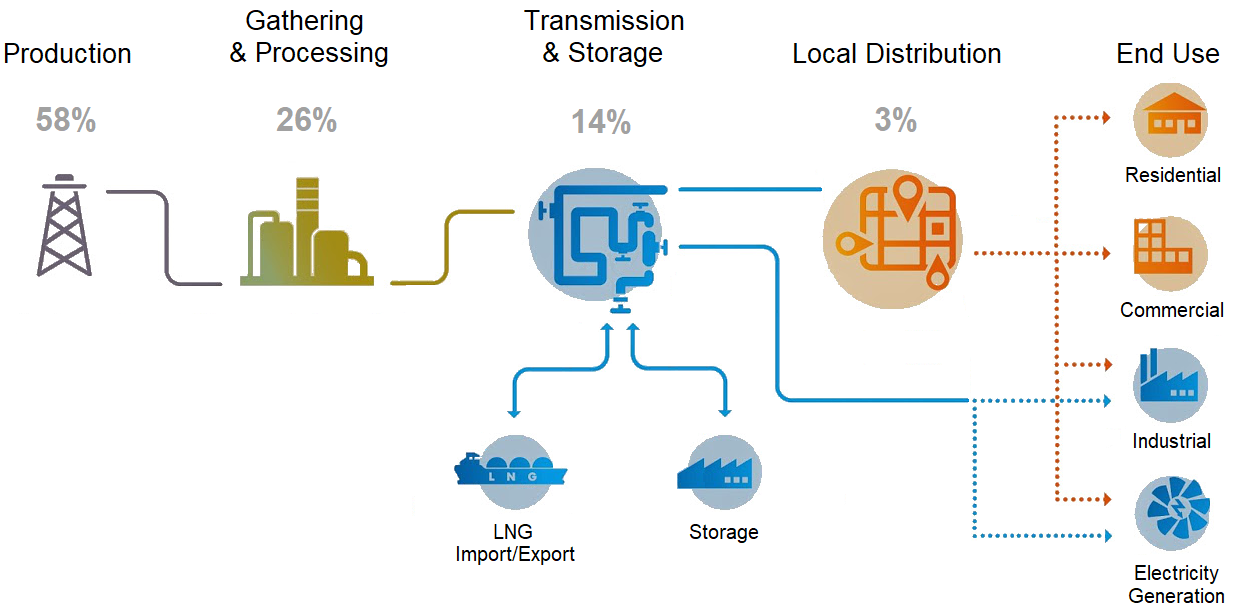
\includegraphics[width=\textwidth]{natural_gas_leakage_percentages_marks_fig1}

\textsc{Source:} \textcite{Marks:2021} figure~1, from estimates in \textcite{Alvarez/etal:2018}.
Excludes end-use leaks.
\end{figure}

\begin{table}[!bth]
\centering
\import{individual_figures/}{Cusworth_etal_2019_table2.tex}
\end{table}


\begin{figure}[!bth]
\caption{Distribution of detected methane leaks, comparison with ground-based measurement}
\label{fig:app-leak-sizes}
\includegraphics[width=0.5\textwidth]{leak_comparison_sizes}
\includegraphics[width=0.5\textwidth]{leak_comparison_fraction_with_detections}

\textsc{Left:} emissions conditional on detection.
\textsc{Right:} fraction of well pads with detected emissions.
The ``ground cens at'' columns are the ground studies' observations with artificial censoring applied, at either 5~or 10~kg/hr, the approximate detection threshold of both the California and Four Corners studies.
Without artificial censoring, the ground-based measurements are non-zero approximately 97\% of the time.
% Unrounded: 96.73913%
5~kg/hr is noted with a dashed line in the left plot.

\textsc{Sources:}
Ground studies include measurements primarily from
\textcite{Robertson/Edie/Snare/Soltis/Field/Burkhart/Bell/Zimmerle/Murphy:2017}
with additional contributions from
\textcite{
Rella/Tsai/Botkin/Crosson/Steele:2015,
Omara/Sullivan/Li/Subramanian/Robinson/Presto:2016,
Omara/Zimmerman/Sullivan/Li/Ellis/Cesa/Subramanian/Presto/Robinson:2018,
}.

California and Four Corners distributions come from aircraft studies \parencite{Duren/etal:2019, Frankenberg/etal:2016}.
\textcite{Lyon/Alvarez/Zavala-Araiza/Brandt/Jackson/Hamburg:2016}
provides information about leak prevalence (with a detection threshold roughly similar to the California and Four Corners studies), but not leak size.
\end{figure}



\begin{table}[!bth] % \ref{tab:covariate-balance-comparison}
\import{individual_figures/}{covariate_balance_comparison_detect_leak.tex}
\end{table}


\begin{figure}[!hbt] % \ref{fig:frankenberg-measurement-figs}
\import{individual_figures/}{frankenberg_measurement_figs.tex}
\end{figure}


\begin{figure}[!hbt] % \ref{fig:nat-gas-price-timeseries}
\import{individual_figures/}{nat_gas_price_timeseries.tex}
\end{figure}



\ifthenelse{\boolean{endfloat}}{}{\FloatBarrier} % add a \FloatBarrier if not using endfloat


\newpage

\section{Distribution Fitting}
\label{app:distribution-fitting}

\begin{table}[!bth]
\centering
\import{individual_figures/}{model_parameters_leak_size.tex}
\end{table}

\begin{table}[!bth]
\centering
\import{individual_figures/}{model_parameters_obs_leak.tex}
\end{table}

\ifthenelse{\boolean{endfloat}}{}{\FloatBarrier} % add a \FloatBarrier if not using endfloat


\newpage
\section{Drilling Response Details}
\label{app:drilling-response-details}

We consider the extensive margin: wells that face some fee for their emissions will see lower profits, all else equal, than wells that face no fees.
Therefore, fewer wells will be drilled.
(It is unlikely that existing wells will stop producing, or that wells will change the amount they produce; \cite{Anderson/Kellogg/Salant:2018}.)
To keep things simple, we assume that there's no change in the composition of wells drilled.

To estimate an approximate drilling response, we first translate our expected fees into profit-equivalent changes in the price of natural gas, then we use estimates from the literature of the elasticity of drilling with respect to price.
Further, we assume that a well's cost of drilling does not change in this scenario, except for the cost of abatement.
We also assume that the policy does not lead to any change in the commodity price of natural gas.

To define some notation, say that without any methane policy a well operator spends $D$ to drill a well, and implement the privately optimal level of abatement.
They earns $E p_0$ revenue on the well's operation.
Here we elide complications like prices changing over time, uncertainty, and discounting.%
\footnote{%
Here we rely on a martingale price assumption, that today's price is the best guess for tomorrow's price.
Ignoring discounting is less of a problem than it would seem because we consider a change in price that applies to every future period, just as the expected change in profits applies in every future period.
}
With under an audit policy, they still spend $D$ to drill the well, but now they also spend an additional $C$ on abatement and $F$ on expected fees.
Revenue is now $(E + \epsilon) p_0$, since some additional gas may be captured.
We define the profit-equivalent price change as the (lower) price that would result in the same profit the well would earn under the no-policy case.
The profit-equivalent price change is:
\[
\Delta p = \frac{C + F - \epsilon p_0}{E}
\]
We have all the pieces to calculate this.
For this calculation, we consider considering \ref{policy-target-e}b), which uses remote measurements to target leaks and a realistic detection threshold.
Using the highest fee we considered ($\tau = 2\delta$ and $T$ = 3 months),
we find the production-weighted average price-equivalent is
\import{tex_fragments/}{OUTCOME=net_private_cost_per_mcf_pct_price_RULE=target_e_high_FRAC=1pct_tauT=high-3month.tex}\%
of the wholesale prices in our sample (which are approx. \$2.90--3.90).

We then turn to the price elasticity of drilling.
We rely on \textcite{Gilbert/Roberts:2020}, which calculates that the production-weighted long run elasticity of gas drilling with respect to the Henry Hub gas price is about 0.36 for all onshore drilling in the continental US, or 0.93 for their five-basin focus.
\footnote{%
In table 6 of that paper, the authors report the continental US short-run elasticity of 0.17 (s.e. 0.096), with the coefficient on the lagged dependent variable of 0.53 (s.e. 0.96).
We calculate the approximate long-run elasticity as 0.36 (\hbox{= 0.17 / (1 $-$ 0.53)}).
}

Combining these, we come to the conclusion presented in the main text.
Even a high-fee policy would see at most a 5--10\% reduction in new (production weighted) drilling, and therefore the changes in expected emissions from this margin are small.

% Cites from the appendix:
% \printbibliography[heading=subbibliography, title={Appendix Citations}]
\end{refsection}

\newpage

\begin{refsection}[software_cites_r.bib,software_cites_python.bib]
\singlespacing
\twocolumn
\nocite{*}
\printbibliography[heading=subbibliography, title={Software Citations}]
\end{refsection}
\end{document}
